\documentclass[12pt,a4paper]{report}

\usepackage{graphics}
\usepackage{fullpage,epsf,graphicx}
\usepackage{amsmath}%, amstext,url}
\usepackage{comment}
\usepackage{hyperref}
\usepackage{verbatim}
\usepackage{float}
\usepackage{placeins}
\usepackage{subcaption}
\graphicspath{{figures/}}
\def\BibTeX{{\rm B\kern-.05em{\sc i\kern-.025em b}\kern-.08em
    T\kern-.1667em\lower.7ex\hbox{E}\kern-.125emX}}

\begin{document}

\thispagestyle{empty}

%
%	This is a basic LaTeX Template for the TP/MP MSc Dissertation report

\parindent=0pt          %  Switch off indent of paragraphs 
\parskip=5pt            %  Put 5pt between each paragraph  

%	This section generates a title page
%       Edit only the sections indicated to put in the project title, and submission date

\vspace*{0.1\textheight}

\begin{center}
        \huge{\bfseries Event Attribution}\\ % Replace with the title of your dissertation!
\end{center}

\medskip

\begin{center}
        \Large{Christopher Long}\\  % Author of dissertation - replace with your name!
        \medskip
        \large{August 18, 2023}  % Submission date
\end{center}

%%% If necessary, reduce the number 0.4 below so the University Crest
%%% and the words below it fit on the page.
%%% Don't let the crest, or the wording below it, flow onto the next page!

\vspace*{0.4\textheight}

\begin{center}
        
\includegraphics[width=35mm]{crest}
\end{center}

\medskip

\begin{center}

\large{
  MSc in Mathematical Physics\\[0.8ex]
  The University of Edinburgh\\[0.8ex]
  2023}

\end{center}

\newpage


\pagenumbering{roman}

\begin{abstract}

Extreme rainfall on 12 August 2020 caused the Stonehaven Derailment,
    which resulted in three deaths.
This project applies current event attribution techniques for extreme rainfall events,
    finding a probability ratios for the extreme rainfall to be 1.1, 1.3 and 1.6 for the 1980s, 2010s and in a 2K warmer world
    respectively over pre-industrial.

\end{abstract}

\pagenumbering{roman}

\begin{center}
\textbf{Declaration}
\end{center}

I declare that this report is entirely my own work unless stated otherwise.

The introduction, chapter~\ref{ch:intro}, describes the motivations for the work.
This includes the information showing the impact of the extreme rainfall on the derailment by the Rail Accident Investigation Board~\cite{RAIB_2022},
    as well as my supervisor's paper analysing the effect of climate change on the risk of an extreme rainfall event~\cite{Tett_Soon}.

Chapter~\ref{ch:attribution} contains background material,
    with the first and third sections primarily relying on World Weather Attribution's methodology~\cite{van_Oldenborgh_et_al_2021},
    and the second section makes use of the information in Coles' textbook on the topic~\cite{Coles_2001}.

Chapter~\ref{ch:dev} consists of my own work,
    excepting the use of code and creation of equivalent diagrams to a currently approved but not yet published paper by my supervisor.
Code used in this project is given in~\cite{Me_Code},
    code used in my supervisor's paper is given in~\cite{Tett_Code}

Chapter~\ref{ch:results} is entirely my own work.

\bigskip

Calculations used Python with many standard packages.

NumPy and XArray are used to manage and process both real and modelled rainfall data.

CartoPy is used to process data between both Ordinance Survey and Longitude-Latitude coordinate systems.

R and the RPy package are used to fit extreme value distributions to the rainfall data.
This calls the extRemes R package~\cite{extremes_R}.

The Rain Radar Data is taken from the Met Office's NIMROD system~\cite{radar_data}.

The Model Data is taken from the Met Office Hadley Centre's UKCP18 Convection-Permitting Model projections~\cite{model_data}.

Tht topography data on an OSGB grid is taken from~\cite{radar_topog}.

The data processing ran on both the JASMIN supercomputer and on my local machine,
GitHub was used to manage the transfer of both code and data.

The majority of the code used in this project is based on the code used by my supervisor performing a similar analysis on the 2021 Edinburgh cloudburst~\cite{Tett_Soon}.


\newpage

\begin{center}
\textbf{Personal Statement} % Use Git commits
\end{center}

I spent the first 2 weeks of the project retro-fitting the Edinburgh castle
library to apply to the Stonehaven crash.
This process began by creating plots including the
rainfall at the crash location on the day and an animation of the rainfall
in the Stonehaven region, allowing me to find an appropriate event definition.

For the remaining weeks of June, I implemented a topographical height mask
to the radar data, as well as establish a workspace to transfer data between
my laptop and the JASMIN supercomputer.

Following this I began my analysis of the radar data.
This involved computing and plotting the monthly rainfall maxima in
the Stonehaven region, as well as finding the quantiles of these extrema,
as well as using R to find the parameters of a GEV fit to both the empirical
and a monte carlo bootstrap of the rainfall distribution.

In mid-July, I created plots for these distributions and started to work with the Convection Permitting Model data,
    processing it as necessary to be appropriate for the use case.
This allowed me to create the time series to act as covariates to the CPM rainfall data,
    which were used in the first week of August to compute the probability ratios, intensity ratios and plots.
Any work done in August other than writing up the dissertation was spent analysing and critiquing the techniques used.

I started writing this dissertation in mid-July, and I spent the first
three weeks of August working on it full-time.

I have achieved the final outcome of probability ratios for the event and
    discussed the limitations of these results.


\newpage

\begin{center}
%\vspace*{2in}
% an acknowledgements section is completely optional but if you decide
% not to include it you should still include an empty {titlepage}
% environment as this initialises things like section and page numbering.
\textbf{Acknowledgements}
\end{center}

I'd like to thank my supervisor Professor Simon Tett for
making this project possible.



\tableofcontents
\listoftables
\listoffigures

\pagenumbering{arabic}

\chapter{Introduction}\label{ch:intro}

\section{Stonehaven Derailment}\label{sec:stonederail}

%  TODO use RAIB analysis

\section{Rainfall in a warmer world}\label{sec:warmerrainfall}

%  TODO rely on Simon's paper and other references
\begin{comment}
The Introduction should contain a description of your project and the
problem you are trying to solve. It should start off at a level that
should be understandable by anyone with a degree in physics, but it
can become more technical later

Where appropriate you should include references to work that has
already been done on your topic and anything else which lets you set
your work in context.
\end{comment}

\chapter{Event Attribution Theory}\label{ch:attribution}
As a part of a complex system,
    any weather event is necessarily multifactorial,
    with no single cause.
It is therefore necessary to use a probabilistic lens to perform a scientific analysis.

In this case, the weather at a given place and time of year is expressed as a statistical distribution of events.
The climate may then be considered either the distribution itself,
    or the parameters informing the distribution.
In other words, ``Climate is what we expect, weather is what we get.''~\cite{Herbertson_1935}.

The scientific method may then be applied,
    using the climate distribution as a dependent variable to the factor being considered.
Issues, of both a technical and a theoretical nature can arise with this approach,
    and will be discussed in subsection~\ref{sec:attrchallenge}.

In all the examples given in this section,
    the independent variable is anthropogenic climate change.
This is often quantified by using a temperature metric,
    although additional factors may be considered.

It may be noted that,
    due to their generality,
    climate event attribution techniques may be of use outside risk analysis from modern changes in the climate.
For example,
    Ruddiman~\cite{Ruddiman_2010} has attempted to attribute the lack of a recent glaciation to the beginning of agriculture.

An event attribution study aims to provide two quantities.
The first is the change in the probability of the event.
The second is the change in the intensity of the event.

\subsubsection{Development of Event Attribution}

In 2003, whilst experiencing flooding as a result of extreme weather,
    Allen~\cite{Allen_2003} posited the probabilistic interpretation of climate change impacts,
    proposing a potential to find greenhouse gas emitters liable for extreme weather events.
%  Add note about the fact that a grant would not be paid to emitters for reducing the likelihood.
A notable early use case of this probabilistic approach was by Stott et al.~\cite{Stott_2004},
    finding that 75\% of the risk of the European heatwave is attributable to anthropogenic climate change.

World Weather Attribution produces rapid Event Attribution studies,
    some of which are within a month of the event occuring~\cite{van_Oldenborgh_et_al_2018},
    using the probabilistic approach.
Alternative approaches also exist.
One of these is the `Boulder' methodology,
    described in section 2.2 of~\cite{Otto_2017},
    which seeks to break down the proportions to which the event was caused by natural variability and the due to Anthropogenic Climate Change.
Another is the `storyline' methodology,
    outlined by Shepherd et al.\ in~\cite{Shepherd_et_al_2018},
    although this has been considered contentious~\cite{García-Portela_Maraun_2023}.

\section{Steps to Event Attribution}\label{sec:attrsteps}

The precise number of steps for successful event attribution vary by the situation.
Van Oldenborgh et al.~\cite{van_Oldenborgh_et_al_2021} give 8 separate steps,
    while Otto~\cite{Otto_2017} gives 6 steps.
Both of these methodologies are functionally identical;
    I shall base my description upon 4 of the steps described by Otto.

Only four steps are given in full below.
This is due to the removal of an analysis trigger step at the start of the process
    and a communication step at the end of the process,
    both of which I will cover here briefly.

An analysis trigger is a set of criteria used to determine whether an event should be investigated.
These serve a utilitarian purpose,
    allowing the events with the greatest impact to be investigated first.
These may include the number of deaths or number impacted,
    as in chapter 2 of~\cite{van_Oldenborgh_et_al_2021},
    or economic and cultural factors, as in~\cite{Tett_Soon}.
The former criteria may skew analysis towards poorer nations~\cite{Kahn_2005},
    while the latter may skew analysis towards richer nations.

It is of note that potential liability of anthropogenic climate change may be a triggering factor,
    so the analysis begins due to a hypothesis that the event was caused by anthropogenic climate change.
I believe that this may bias the results of a meta-analysis of event attribution studies,
    and so increase the challenge in determining anthropogenic climate change as a cause of more extreme events in general.
I omit giving any further detail on the analysis trigger as it is beyond the scope of mathematical or physical interest.

The communication of the outcome of the analysis may also be considered in the study.
This is especially true outside the scientific community
    and considers the risk of the audience drawing incorrect conclusions,
    as well as the risk of policymakers acting on incorrect information.

\subsection{Event Definition}\label{subsec:backeventdef}

To perform an attribution analysis,
    the weather event must first be defined in clear and quantitative terms.
This requires specifying a variable with a threshold that has been crossed,
    as well as the time and region at which an event may be considered.

This is not necessarily straightforward.
An event attribution is normally triggered by the event's social or environmental impact,
     not just due to the meteorological significance.
Therefore, care must be taken to ensure that the definition of the event is sufficiently similar to the conditions that would cause a similar impact.

Many of the challenges in Event Attribution arise directly from a poor Event Definition.
Events that are too narrowly defined may have issues with reproducibility,
    as will be discussed in~\ref{subsec:eventrepro},
    while events that are too widely defined may give invalid results,
    as will be discussed in~\ref{subsec:modelvalid}.

\subsubsection{Variable and Threshold}

The climate variable used to define the event requires travelling up the causal chain that leads to it.
As a set of examples,
    floods/droughts are caused by extreme highs/lows in rainfall,
    while heat waves and cold spells are caused by extreme high or low temperatures.

However,
    all of these events require the extreme rainfall/temperature to be sustained for the event to be hazardous.
Simple metrics may be applicable here,
    as the definition can then use the rainfall/temperature averaged over a given time period.
The selection of time period itself also requires a consideration of the event.
A damaging heavy storm requires extreme winds over a matter of minutes,
    while it may take days for the land to dry out sufficiently for a drought to occur.

More advanced metrics may be used.
For example, an Expert Team on Climate Change Detection Indices~\cite{Zhang_2011}
    describes a `Growing Season Length',
    allowing climate-caused famine to be quantified using only daily temperature data.
A `Wet-Bulb Temperature' has been used to combine humidity and temperature data to create an index that better measures teh effect of a heatwave on human health~\cite{Li_2020}.

\subsubsection{Spatial and Temporal Region}

In addition to defining a threshold variable,
    it is necessary to define the regions and times at which an event can be considered sufficiently similar to that being analysed.
This is due to the fact that both historical trend analysis is impossible on a single extreme event at a single place on a single day of the year
    and that climate models will rarely reproduce events in such a narrow definition.
The second of these factors will be discussed in subsection~\ref{subsec:eventrepro}.

For the spatial region,
    a region with a known climate similar to that in which the event occurred is chosen,
    typically directly around the location of the event.
This is done so that the frequency and types of event will match the location of the original event,
    as well as to ensure that the factors that change the climate,
    whether Anthropomorphic or not,
    are similar to those changing the climate at the point of the event.

In addition to the aforementioned similarity in location,
    a historical trend analysis can aid in defining a region,
    along with tools including topography and climate classifications.
The region is chosen based on similar weather,
    not a similarity in hazard risk,
    as the goal is to perform an attribution for the event,
    not to advise on potential future risk.
For example,
    a region defined for a flood event over a flood-prone area would only consider areas with similar rainfall,
    not those similarly flood-prone.

For the temporal region,
    or time period for the event to be considered,
    an analogous process must be used.
It is often appropriate to use a seasonal time period,
    as this can also limit the event to those with similar meteorology,
    such as by only considering monsoon rainfall~\cite{Otto_et_al_2023}.
This can also prove to be a practical step,
    reducing the amount of data to be used later in the attribution process.

Additional `Boundary Conditions'~\cite{van_Oldenborgh_et_al_2021} may then also be imposed.
Of note is the importance of the El Niño,
    especially for drought events in the southern hemisphere~\cite{Lyon_2004},
    so this may also be accounted for when defining these event.

Once all of these definitions have been made,
    a `class' of events has been described.
This class will then be used to find like events in both the historical and model data.

\subsection{Model Evaluation}\label{subsec:backmodeleval}

\subsection{Likelihood Estimation}\label{subsec:backlikeest}

\subsection{Interpretation}\label{subsec:backinterp}

\section{Extreme Value Statistics}\label{sec:exstats}

This subsection will describe the statistical foundations of extreme event modelling,
    paraphrasing Coles' book~\cite{Coles_2001} unless where otherwise stated.
Climate events that pose hazards are necessarily extreme.
Therefore, to model these events,
    extreme value distributions are necessary.

Throughout the analysis,
    we assume that the variables are independent and identically distributed ($i.i.d.$).
The issues that may arise from this assumption not being valid are considered in subsection~\ref{subsec:statvalid}.

For event definitions which average a variable over a season,
    as opposed to focusing on the extreme
    a normal distribution is instead appropriate.
This is as the Central Limit Theorem states that the limit of the mean of $n$ $i.i.d.$ random variables tends to a normal distribution.
The equivalents for extreme events, the GEV distribution and Extremal Types Theorem,
    will be explained in due course.

\subsection{GEV Distribution}\label{subsec:gev}

\subsubsection{Extremal Types Theorem}

This explanation is as given in section 3.1 of~\cite{Coles_2001}.

Let $M_n$ be the maximum of $n$ $i.i.d.$ random variables.
If there exist sequences of constants $a_n > 0$ and $b_n$, and non-degenerate $G$ such that:

\[ P\left( \frac{M_n - b_n}{a_n}  \leq z \right) \rightarrow G(z) \text{ as } n \rightarrow \infty \]

Then $G$ is a member of the GEV (Generalised Extreme Value) family.

Section 3.1.4  of~\cite{Coles_2001} outlines a proof of the Extremal Types Theorem.
This involves showing that being a GEV distribution is equivalent to being `Max-Stable',
    then that the maxima of GEV distributions are Max-Stable,
    giving the GEV as the distribution of the original maximum in the infinite limit.
It is of note that this is similar to one approach to proving the Central Limit Theorem,
    which considers the normal distribution as a unique fixed point under convolutions,
    resulting in normal distributions being an infinite limit of the sum or mean~\cite{Hamedani_Walter_1984}.

Section 3.5 of~\cite{Coles_2001} shows, \textit{mutatis mutandis},
    that the extremal types theorem applies identically to minima by reversing the sign of the data.

\subsubsection{Parameters and Types of GEV distributions}

The GEV distribution has a CDF given by:
\begin{equation}\label{eq:gevcdf}
    G(z) = \exp \left( - \left( 1 + \xi \left( \frac{z-\mu}{\sigma} \right)  \right)^{-\frac{1}{\xi}} \right)
\end{equation}

This has three parameters, the location $\mu$, the scale $\sigma$ and the shape $\xi$.
It is clear from this CDF that the change of location and scale parameters represent moving and rescaling the distribution,
    much as the mean and standard deviation parameters do for a normal distribution.

$1-G(z)$ is the survival function of the distribution.
This function gives the probability of an interval containing an event more extreme (of larger intensity) than $z$.

The shape parameter determines the thickness of the tail of the distribution.
The larger the shape parameter, the thicker the tail of the distribution.

%  TODO insert graph w different shape parameters

Where $\xi > 0$,
    the distribution is heavy-tailed.
This type of GEV distribution is also known as a Fr\'{e}chet distribution.
Special cases of this distribution have unique properties,
    where $\xi \geq \frac{1}{2}$, the distribution has infinite variance and
    where $\xi \geq 1$, the distribution has infinite mean.

Where $\xi < 0$, the distribution is bounded,
    also known as a reversed Weibull distribution.
These distributions are limited to a maximum `most extreme' value of $\mu - \frac{\sigma}{\xi}$.
It can therefore be expected that distributions modelling extrema with physical constraints would have a negative shape parameter.
For example, Table 3 of Chikobvu and Chifurira's paper~\cite{Chikobvu_2015} modelling rainfall minima finds a negative shape parameter,
    which would be expected as rainfall cannot be negative.

Where $\xi = 0$,
    the distribution is a Gumbel distribution.
The CDF of this distribution requires taking the limit as $\xi \rightarrow 0$,
    giving a double exponential CDF\@.
The extrema of normal distributions converge to a Gumbel distribution,
    shown as a step in the proof of Proposition 1 of~\cite{Bailey_2014}.
This means that, with the Central Limit Theorem,
    the maxima of a sample of means of any distribution approaches a Gumbel distribution as both samples grow larger,
    provided the samples are independent.

The above paragraph suggests that a Gumbel distribution is appropriate for modelling rainfall maxima,
    as the rainfall is averaged over a time period and then a maxima is taken over those time periods for a given year or season.
However, this has not been found to be true.
Koutsoyiannis~\cite{Koutsoyiannis_2003} finds both an ``extremely slow'' theoretical convergence to a Gumbel distribution and
    that the Gumbel distribution does not fit empirical rainfall maxima.
Therefore, the three-parameter GEV distribution is used to model rainfall maxima in event attribution.

\subsubsection{Return levels of GEV distributions}

Equation~\ref{eq:gevcdf} can be inverted to give a return level $z_p$ for a probability $p$, given in~\cite{Coles_2001}:
\begin{equation}\label{eq:gevreturn}
    z_p = \mu - \frac{\sigma}{\xi}\left( 1-\left( -\log\left( 1-p \right) \right)^{-\xi} \right)
\end{equation}
This is otherwise known as the inverse survival function,
    where $z_p$ is the value for which the probability of finding a value greater than $z_p$ is $p$.

This can also be used to compute the rarity of events for a return period $P$,
    as the probability $p$ is equal to $1/P$.

This is allows the GEV distribution to use the language common for extreme weather events,
    as with knowledge of the underlying distribution,
    it is possible to compute the intensity of an event for any return period.

\subsection{GEV Parameter Estimation}\label{subsec:parameterest}

In sections~\ref{subsec:radardatafit} and~\ref{subsec:radardatafit},
    parameters are fitted to data using the extRemes R library~\cite{extremes_R}.
This software uses MLE (Maximum Likelihood Estimation) to get best estimates of the parameters of a dataset,
    assuming the data obeys a GEV distribution.
This technique will be covered briefly here.

The extRemes package is also used to fit linear changes in a parameter with respect to a covariate.
Although this uses the same underlying mathematics as this section,
    relying on MLE,
    the exact algorithm used is beyond the scope of this report.

\subsubsection{Maximum Likelihood Estimation}

\subsubsection{Akaike Information Criterion}

To assess the goodness of fit,
    the Akaike Information Criterion (AIC)~\cite{AIC_1974} is used.
This is given in the following equation:
\begin{equation}\label{eq:AIC}
    AIC = 2k - 2\ln \left( L \right)
\end{equation}
Where $k$ is the number of parameters and $L$ is the value of the likelihood function with the data.

A better fit has a lower AIC .
Equation~\ref{eq:AIC} imposes a cost of 2 per parameter,
    preventing overfit models with many parameters being considered a good fit for the data.

For Models 1 and 2, the probability that model 2 loses less information than model 1,
    i.e. that model 2 is a better fit than model 1,
    is given in~\cite{AIC_Info}:
\begin{equation}\label{eq:AIC_Info}
    \exp \left( \frac{1}{2} \left( AIC_1 - AIC_2 \right) \right)
\end{equation}

\section{Challenges in Event Attribution}\label{sec:attrchallenge}

\subsection{Event Reproducibility}\label{subsec:eventrepro}

\subsection{Statistical Reliability}\label{subsec:statvalid}

\subsection{Validity of Model}\label{subsec:modelvalid}

\chapter{Development}\label{ch:dev}

Throughout this chapter,
    reference is made to the `Stonehaven Region'.
This is defined as +/- 50km of the crash location for empirical data,
    which uses an ordinance survey grid,
    and as +/- 0.5 degrees of the crash location for the model data.

\section{Empirical Data}\label{sec:def}

The data used in this section is taken from the Met Office's NIMROD system~\cite{radar_data}.
This data has a 5km by 5km spatial resolution and a 15-minute temporal resolution,
    although data is also available in a 1km by 1km spatial resolution.
The coarser dataset was chosen as the Stonehaven event was a Summer convective storm,
    which occurs on scales great enough to be captured at a 5km resolution.

\subsection{The Stonehaven Event}\label{subsec:actualevent}

\subsubsection{Rainfall at the crash location}

\begin{figure}[H]
    \begin{center}
    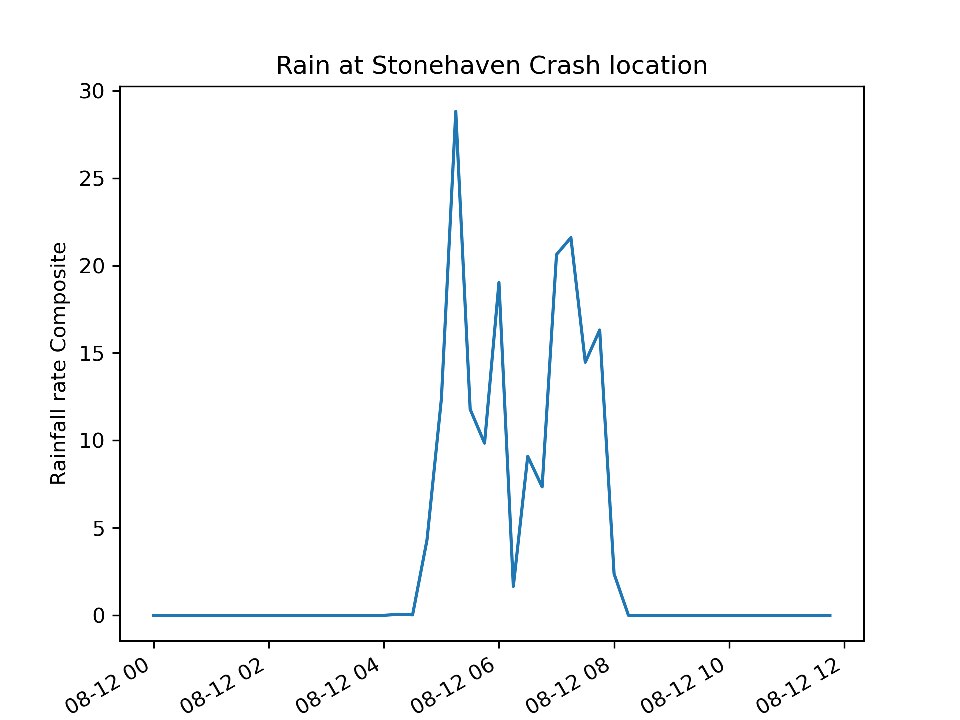
\includegraphics[width=100mm]{stonehavendayraingraph}
    \end{center}
    \caption[A graph of the rainfall at the Stonehaven crash location.]{
        A graph of the rainfall at the Stonehaven crash location.
    X-axis is the date and hour (24-hour clock) of the rainfall measurement,
        ranging across the morning of the 12th of August 2020.
    Y-axis is the rainfall measured in mm/h.}
    \label{fig:stonehavendayraingraph}
\end{figure}

From Figure~\ref{fig:stonehavendayraingraph},
    the rainfall event begins at 4:15 and ends at 8:15.
The rainfall at the crash location is then given in sixteen 15-minute chunks of time,
    or as across four hours.

This may suggest a four-hour event definition should be used.
However, this was not done for two reasons.
First, it is clear that the rainfall occurred in two 2-hour peaks,
 so a 4-hour definition may not be appropriate for this event.
Second, in section~\ref{subsec:radarprocess},
    the radar data is processed into chunks,
    each of which starts on an increment of the length of time of the event.
While this would accurately capture this 4-hour storm, being between 4:00 and 8:00,
    an event from 6:00 to 10:00 would be considered two events of half the size.

A one-hour maximum rain definition was used instead,
    as it allowed storms of differing lengths to be quantified by their peak hourly rainfall.

\subsubsection{Rainfall in the Stonehaven region}

\begin{figure}[H]
    \centering

    \begin{subfigure}{0.48\textwidth}
        \centering
        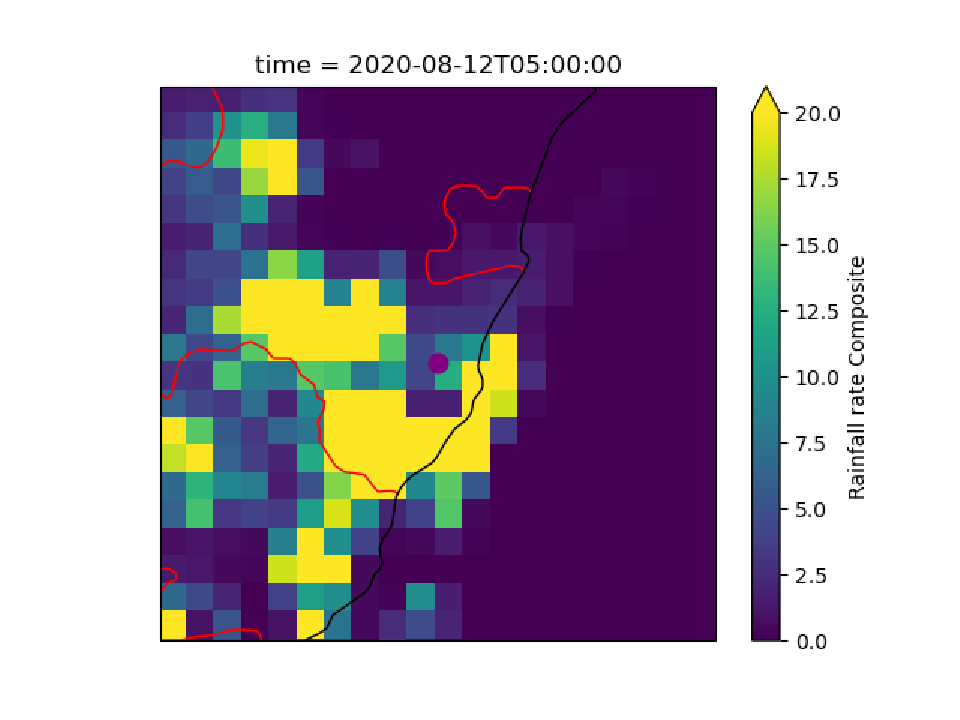
\includegraphics[width=\linewidth]{stonerain5}
    \end{subfigure}
    \hfill
    \begin{subfigure}{0.48\textwidth}
        \centering
        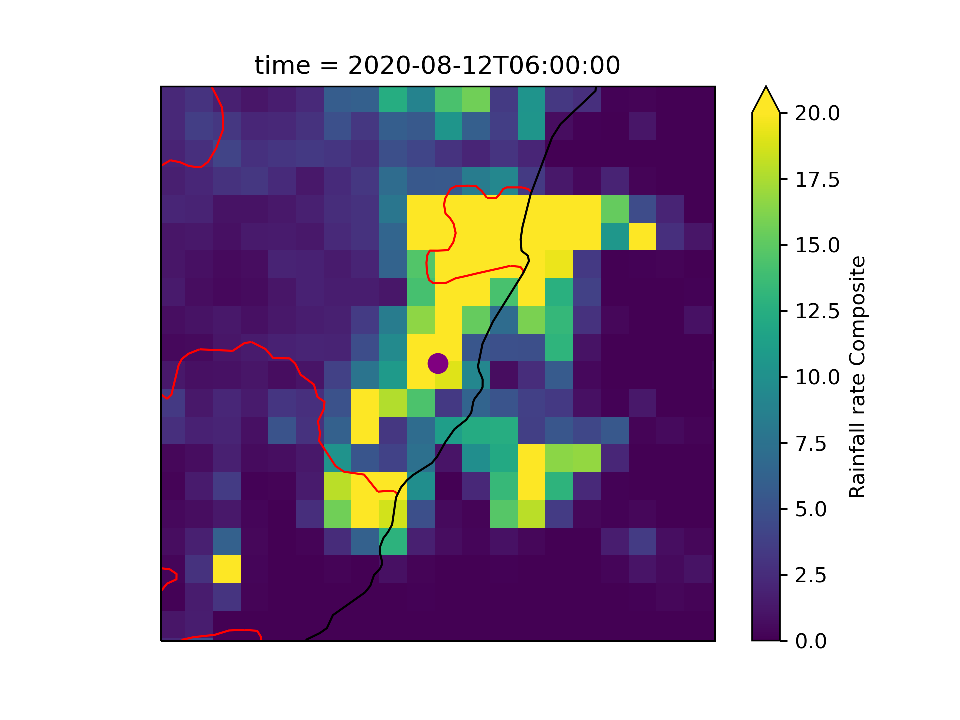
\includegraphics[width=\linewidth]{stonerain6}
    \end{subfigure}

    \vspace{\baselineskip}

    \begin{subfigure}{0.48\textwidth}
        \centering
        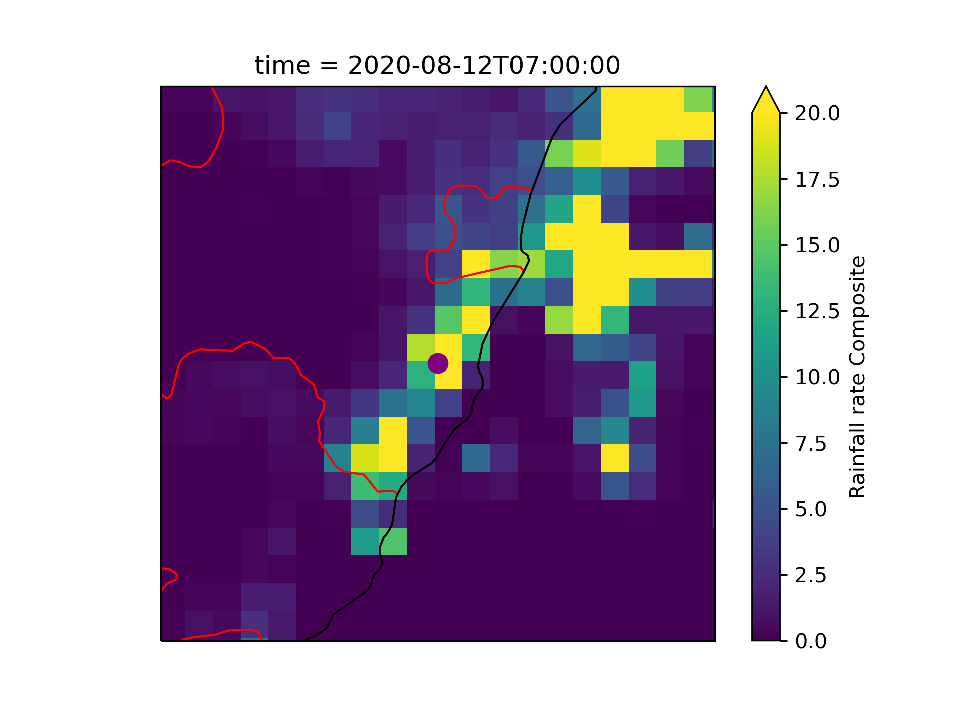
\includegraphics[width=\linewidth]{stonerain7}
    \end{subfigure}
    \hfill
    \begin{subfigure}{0.48\textwidth}
        \centering
        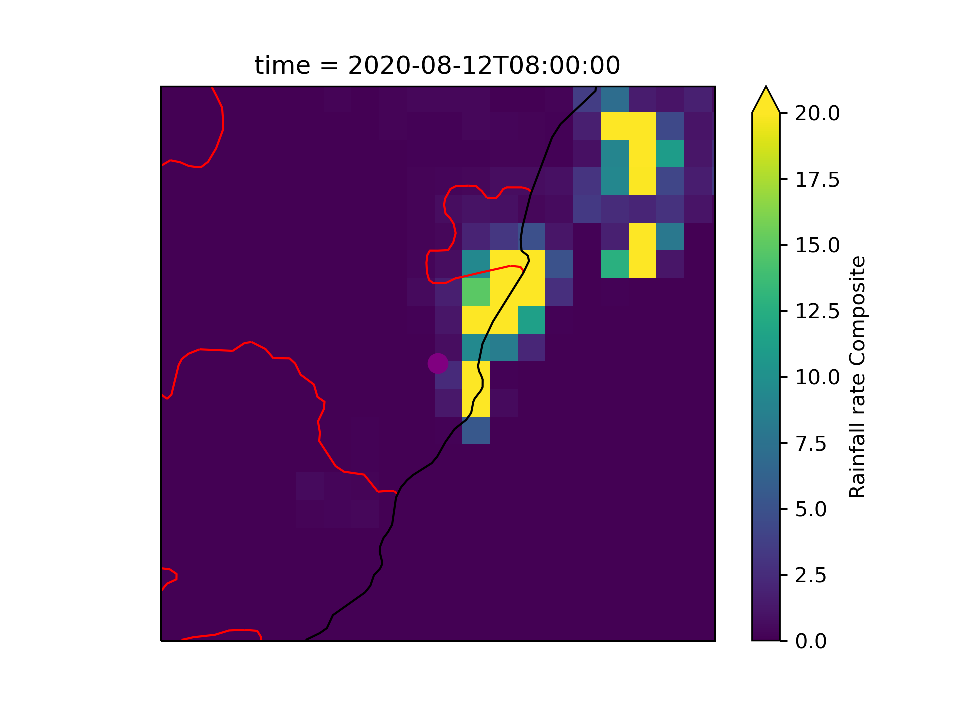
\includegraphics[width=\linewidth]{stonerain8}
    \end{subfigure}
    \caption[Map of rainfall in the Stonehaven region at times in the morning of 12th August 2020.]{
        Map of rainfall in the Stonehaven region (+/- 50km of Stonehaven)
        at times of 5, 6, 7 and 8 AM of the 12th August 2020,
        in the top left, top right, bottom left and bottom right respectively.
    Scale is mm/h.
    Black lines are coastlines, red lines are local authority boundaries.
    Purple dot is the crash location.}
    \label{fig:stoneregionrain}
\end{figure}

Figure~\ref{fig:stoneregionrain} shows the rainfall in the Stonehaven region,
    demonstrating the movement of the storm North-East throughout the morning of the event.
This figure is also available as an animation using data from 15-minute intervals,
    showing the storm moving as expected.

The figure also suggests that the event covers a large area,
    validating the use of the coarser-resolution 5km dataset as sufficient to describe the event.
One unfortunate consequence of using the 5km dataset is on the rainfall described in Figure~\ref{fig:stonehavendayraingraph},
    as the crash location lies near the boundary of four cells, yet the data is only taken from the nearest cell,
    leading to the graph being a less accurate approximation of the rainfall at the crash location than would be given by a 1km resolution dataset.

\subsection{Further Constraints}\label{subsec:furthercons}

\subsubsection{Stonehaven Geography}

\begin{figure}[H]
    \centering
    \begin{subfigure}{0.48\textwidth}
        \centering
        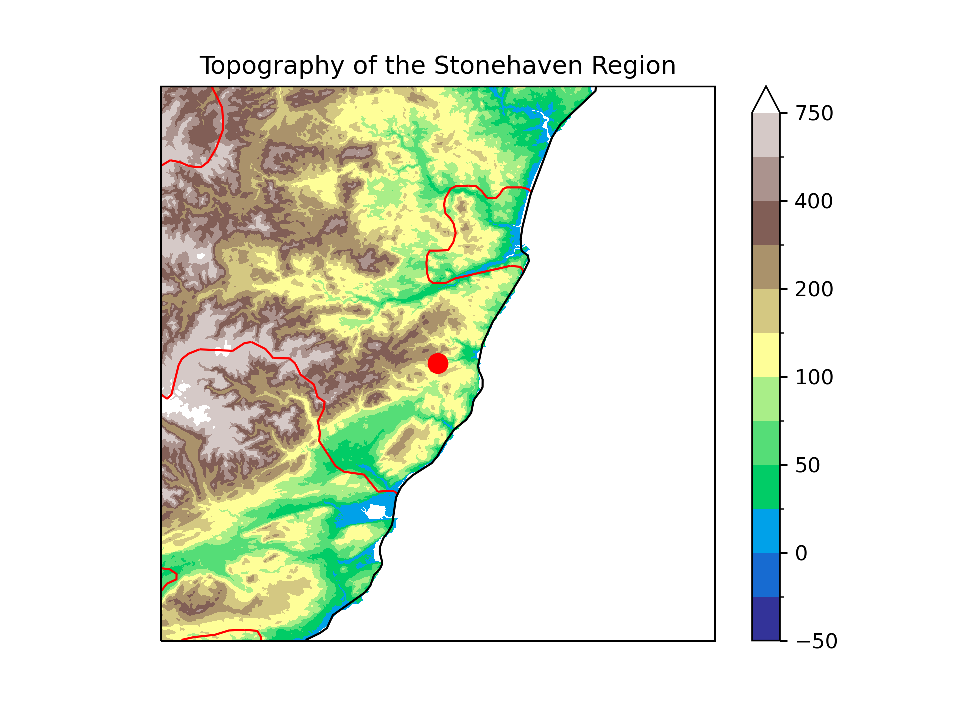
\includegraphics[width=\linewidth]{stonetopog90}
    \end{subfigure}
    \hfill
    \begin{subfigure}{0.48\textwidth}
        \centering
        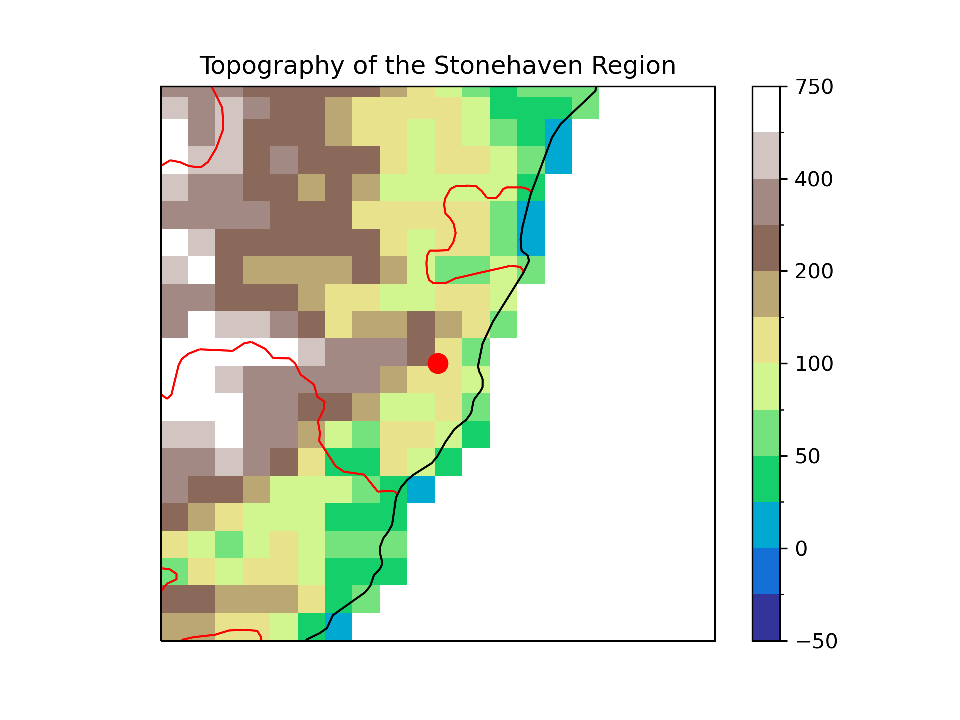
\includegraphics[width=\linewidth]{stonetopog4950}
    \end{subfigure}
    \caption[Plot of the topography in the Stonehaven region.]{
        Plot of the topography in the Stonehaven region.
    Scale is in meters.
    Left is the raw data (at 90mx90m resolution),
    right is the resampled data (at 4950mx4950m resolution) as used for future processing.
    Black lines are coastlines, red lines are local authority boundaries.
    Red dot is the crash location.}
    \label{fig:stonetopog}
\end{figure}

The 4950m resolution data shown in Figure~\ref{fig:stonetopog} was found by taking a mean average of 55 of the data points in each dimension,
    giving each grid cell an average of 3250 raw data points.

The area of the Stonehaven crash is around the 200m contour,
    with the crash occurring at around 100m,
    due to the cutting the railway passes through.
Looking at Figure 26 of~\cite{RAIB_2022},
    the drain responsible for the crash is 150m above sea level.
Furthermore, the drain's catchment reaches close to 200m.

The topography of the region for the event attribution analysis was then chosen to be from 0m (sea level)
    to 400m.
This is done to make the topography around the crash location typical for the region in which the analysis is performed.
A 200m limit was suggested
    to match the limit taken in~\cite{Tett_Soon}
    but was not taken forward as this had the potential to give too few data points to define an event.

\begin{figure}[H]
    \begin{center}
        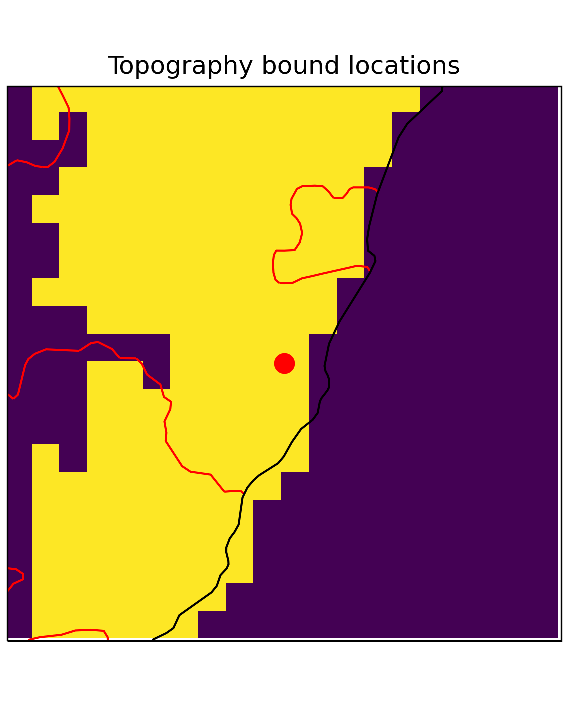
\includegraphics[width=100mm]{stonetopogcut}
    \end{center}
    \caption[Map of the Stonehaven region with radar data grid cells within a range of 0--400m.]{
        Map of the Stonehaven region with radar data grid cells (5kmx5km) within a topographical range of 0--400m in yellow,
    grid cells outside of range in violet.
    Black lines are coastlines, red lines are local authority boundaries.
    Red dot is the crash location.}
    \label{fig:stonetopogallowed}
\end{figure}

Out of the 400 grid cells in the Stonehaven Region,
    data is taken from 185 of the grid cells.
This is as 194 of the grid cells are not over land,
    and an additional 21 grid cells have too high topography.

As the radar data is at a 5km resolution,
    while the resampled topography data is at a 4950m resolution,
    the XArray \texttt{interp\_like} method is used to get a linear interpolation for the height at each 5km grid cell.

\subsection{Processing and Fitting the Radar Data}\label{subsec:radarprocess}

The steps used in this section are identical to those used to process and fit the radar data for the Edinburgh cloudburst event~\cite{Tett_Soon},
    with changes made to fit the different definition and region in this case.

\subsubsection{Computing Maxima}

As the goal was to use an Extreme Value distribution to model the data,
    it is necessary to draw the extrema out from the data.
The dataset itself~\cite{radar_data} is composed of \texttt{.tar} files, each containing the radar data of a given day.

The \texttt{process\_radar\_data}~\cite{Me_Code} Python script finds the maximum one-hour rainfall in each of these daily datasets and
    uses these to generate a dataset with the one-hour maximum rainfall and the time of the one-hour maximum rainfall
    at all points in the Stonehaven Region for a given month, in a NetCDF format
The \texttt{combine\_summary}~\cite{Me_Code} Python script then takes these monthly maxima and their times and combines them into a single dataset,
    again as a NetCDF .

The Shell scripts \texttt{run\_jobs} and \texttt{run\_combine}~\cite{Me_Code} call the above Python scripts respectively.
The Shell scripts are run on a JASMIN Science Analysis Server and submit the Python scripts as SLURM jobs to the LOTUS Batch Processing Cluster,
    allowing all the monthly maxima to be computed in a single script and the combination of the datasets to access an amount of memory to make the task feasible.

The \texttt{get\_radar\_data} function in the \texttt{stonehavenRainLib}~\cite{Me_Code} Python script then selects the summer months and
    combines them to get the maximum hourly rainfall in the summer of each year,
    along with the time of the maxima.
This function also applies the topographical height mask described in subsection~\ref{subsec:furthercons},
    returning an XArray DataSet of the radar data that will be used to describe and generate statistics for the event.

\subsubsection{Computing Events and Definition}

Now that the seasonal maxima have been found,
    the data can be used to define events.
This process is done in the \texttt{gen\_radar\_data} function in the \texttt{stonehavenRainLib}~\cite{Me_Code} Python script.
The seasonal maxima,
    of which there is one for each grid cell in each year in the dataset,
    are grouped by the time in which they occurred.

These groups are 12-hour periods,
    representing either the AM or PM hours of a day.
Each group is then an event,
    containing the grid cells which experienced their maximum hourly rainfall within the group's time period.
The groups with less than 10 grid cells were discarded,
    as these events are less than 250km$^2$ in size and
    so do not represent events similar enough to the Stonehaven event.

This gives a final event definition as 250km$^2$ of the land below 400m and within +/- 50km of Stonehaven
    experiencing their annual summer hourly rainfall maxima in the same 12-hour period.
For each event, the 0.05, 0.1, 0.2, 0.5, 0.8, 0.9 and 0.95 quantiles were found and returned in a dataset.
The intensity of a given event is defined by its 0.95 quantile.

Due to the separation into 12-hour bins,
    it is assumed that each event is independent in all future calculations.

\begin{figure}[H]
    \centering
    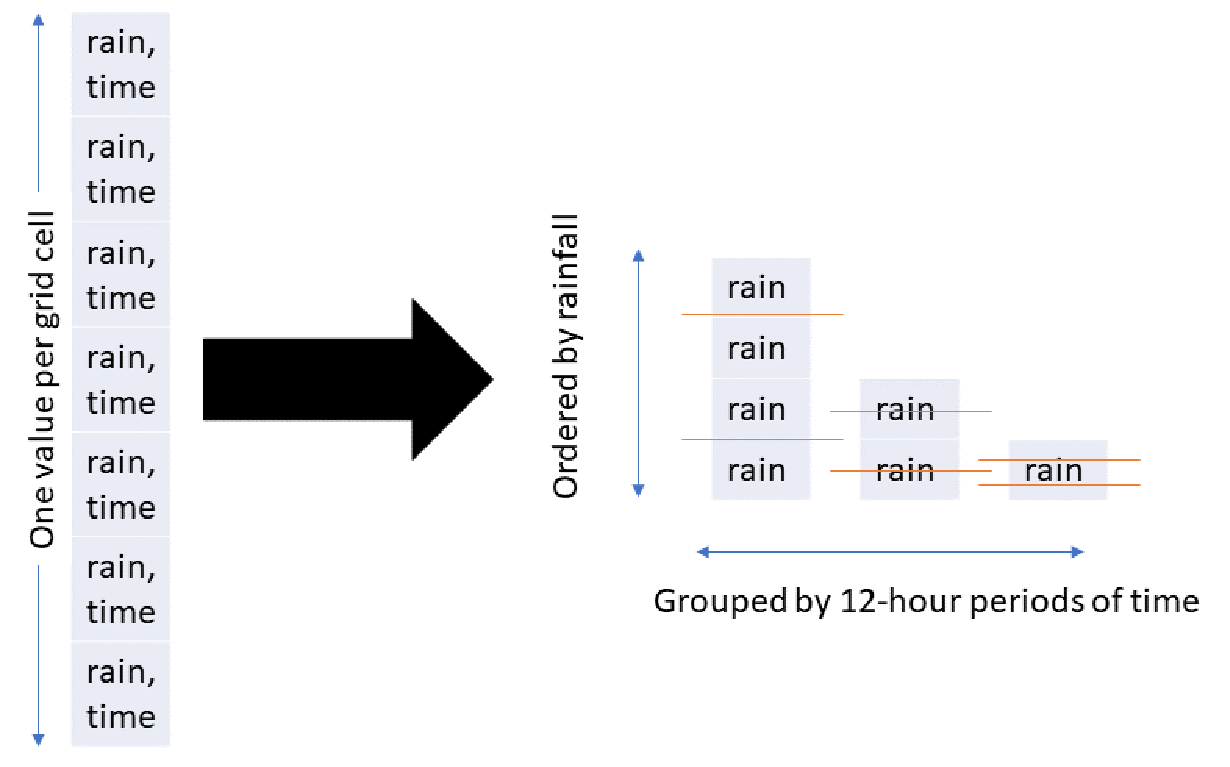
\includegraphics[width=100mm]{dataprocessschematic}
    \caption[Diagram representing the data processing.]{
        Diagram representing the data processing after the maximum of each grid cell has been found,
    within each year.
    `rain' represents the summer maximum rainfall in a grid cell,
        `time' represents the time of this maximum,
        red horizontal lines represent the taking of quantiles from the rainfall maxima.
    Number of data points and quantiles are not to scale.}
    \label{fig:dataprocessschematic}
\end{figure}

\subsubsection{Fitting event distribution}

The radar data is fit to a GEV distribution with the \texttt{comp\_radar\_fits}~\cite{Me_Code} Python script,
    which calls the \texttt{gev\_r}~\cite{Me_Code} Python library to run code in R .
The `fevd', fit extreme value distribution,
    command in R is used to fit an extreme value distribution to the radar data,
    which uses MLE, as described in subsection~\ref{subsec:parameterest}.
This command is applied to each of the quantiles of the event,
    with the events as the data points,
    giving the parameters of GEV distributions describing each quantile of the events.
With these parameters generated,
     it was possible to find the empirical return period for the Stonehaven event.

To generate uncertainties,
    a Monte Carlo bootstrap method is used,
    given in the \texttt{mc\_dist} function.
This involved generating a list of the same size of the number of events,
    taking a random sample with replacement,
    and then applying the `fevd' command to each sample.

1000 samples were taken,
    of which 9 provided anomalous (negative) location or scale parameters,
    and so were discarded.
The discarding process was valid as the value of these parameters was ~-100,
    while all other samples had values of these parameters between 2 and 15,
    as well as that removing such few samples would not have a significant effect on the 95\% confidence interval.
The 991 samples left are greater than the 800 suggested by Booth and Sarkar~\cite{Booth_Sarkar_1998}
    for effective error estimation.

\section{Modelled Data}\label{sec:model}

The model data used in this section is
    the Met Office Hadley Centre's UKCP18 Convection-Permitting Model Projections for the UK at 2.2km resolution~\cite{model_data}.
This dataset was chosen as the resolution is less than 5km,
    and so it is able to represent convective storms directly.

The CPM ensemble consists of 12 members and covers the 100 years from 1981 to 2080,
    modelling the RCP8.5 emissions scenario.
In this investigation,
    the model's hourly temperature and rainfall data will be used.

This model was created by using a 60km resolution global model to impose boundary conditions on a 12km regional model,
    which was then used to impose boundary conditions on the 2.2km model.
The guidance for the model~\cite{model_data} states that the 2.2km model is appropriate for sub-daily extrema,
    so long as the assessment is probabilistic,
    which is done in this analysis.

The model evaluation steps in~\ref{subsec:backmodeleval} are not applied here.
This is as an unusual event definition has been created in section~\ref{sec:def},
    which applying to the model would be beyond the scope of this project.
The model here does not have to represent the event identically as the model data is only being used to gather information
    to apply to the empirical fit,
    not to calculate the risk ratios directly.

\subsection{Pre-processing}\label{subsec:preprocess}

The CPM data used is on longitude-latitude coordinates,
    with the North Pole rotated to near the region the model covers.
The location of the Stonehaven crash in this alternative coordinate system was found using the \texttt{comp\_rotated\_coords}~\cite{Me_Code} Python script,
    using CartoPy for the computations.
This coordinate rotation was also done for the four weather stations used to compute Central England Temperature (CET).

The pre-processing of the CPM data is done using the \texttt{ens\_seas\_max\_coarsen}~\cite{Me_Code} Python script,
    which finds the seasonal one-hour rainfall maxima for each grid cell.

\subsubsection{Coarsening}

The CPM data uses a 2.2km resolution,
    while the radar data uses a 5km resolution.
To account for this,
    the radar data is coarsened using the XArray \texttt{.coarsen} and \texttt{.mean} methods,
    taking the mean average of four 2.2kmx2.2km grid cells, giving 4.4kmx4.4km grid cells.

The height mask for the CPM was in the same 2.2km resolution
    and so required the same pre-processing

\subsubsection{Height mask}

To match the event definition in section~\ref{subsec:radarprocess},
    a similar height mask must be used,
    with the same limits of 0m to 400m.

The CPM used for this study is a projection over land,
    with other UKCP18 models covering the marine domain,
    albeit at a lower resolution of 12km and covering storm surges and sea levels as opposed to precipitation,
    as described in the guidance of~\cite{model_data}.
This makes the >0m height mask on the model a necessity,
    as the model projections over the sea (with height 0m) are invalid.

\subsection{Covariates}\label{subsec:covfit}

\subsubsection{Time Series}

The \texttt{comp\_cpm\_ts}~\cite{Me_Code} Python script was used to compute the time series.
This script takes each month within each ensemble member of the CPM data and computes three values.
These are computed using the 2.2km data without the coarsening or height mask.
First is the Central England Temperature,
    which takes the CPM data's average monthly temperature at the weather stations used to define CET,
    while the other two time series use the average monthly temperature and precipitation in the Stonehaven Region.

Two additional monthly time series were computed in the \texttt{analyse\_cpm\_data\_rolling}~\cite{Me_Code} Python script.
One of these takes the median extreme precipitation across the Stonehaven Region
    using the extrema processed in \texttt{ens\_seas\_max\_coarsen.sh}~\cite{Me_Code},
While another uses the temperature in the Stonehaven Region to find the Saturation Humidity.

The formula used for this is the August-Roche-Magnus approximation to the Clausius-Clapeyron relation~\cite{Alduchov_Eskridge_1996}, given by:
\begin{equation}\label{eq:qsat}
    e_s = 6.112 \exp\left( \frac{17.6 T}{T + 243.5} \right)
\end{equation}
Where $T$ is the temperature in degrees Celsius.

The scaling of the Saturation Humidity with temperature will be described as the Clausius-Clapeyron scaling.
This is as it represents the amount of moisture that the atmosphere can hold,
    suggesting that rainfall should also scale by this amount with a change in temperature.

Each time series had 14400 members,
    with 12 ensemble members providing data for the 1200 months across the 100-year window of the model.
This was then reduced to 3600 data points by only taking the three summer months of each year.

\subsubsection{Fitting Covariates}

\texttt{analyse\_cpm\_data\_rolling}~\cite{Me_Code} performs a linear fit of the Saturation Humidity,
    Stonehaven Region temperature, mean average Stonehaven Region precipitation and mean maximal Stonehaven Region precipitation.
    using the \texttt{statsmodels} Python package's ordinary least squares regression feature.
This provides the change in each of these variables, as well as the uncertainty with $R^2$ coefficients,
    with respect to each fit.

In a method analogous to the \texttt{comp\_radar\_fits} Python script calling the \texttt{gev\_r} library to use R to fit
    a distribution to the radar rainfall extrema in subsection~\ref{subsec:radarprocess},
    \texttt{analyse\_cpm\_data\_rolling} calls the \texttt{gev\_r} library to perform fits on the model rainfall extrema.
This is done with the same `fevd' command in the extRemes R library~\cite{extremes_R},
    except done with the monthly mean CET, total model area temperature, Stonehaven Region temperature and Stonehaven Region humidity as covariates.

For this,
    the location and scale parameters are allowed to change linearly with the variable $x$.
The parameters are then $\mu = \mu_0 + x\mu_1$ and $\sigma = \sigma_0 + x\sigma_1$.
The analysis is then repeated with the shape parameter also allowed to vary in the form $\xi = \xi_0 + x\xi_1$.

In contrast to \texttt{comp\_radar\_fits},
    \texttt{analyse\_cpm\_data\_rolling} does not perform a single GEV fit on a set of events,
    but instead a GEV fit for each grid cell in the Stonehaven region for the CPM .
This far greater number of fits is possible as the CPM data contains data for 1200 summer maxima for each point,
    with each of the 12 ensembles spanning 100 years,
    as opposed to the 18 for the radar data.
A data fit for each grid cell then allows the effect of the location on the CPM rainfall maxima to be analysed.
This data fit is done nine times,
    with either no covariate or the CET, CPM Region temperature, Stonehaven Region temperature or Stonehaven Region saturated humidity as a covariate.
For each covariate, this is performed with and without the shape parameter varying.

The scaling of the parameters $\mu_1 / \mu_0$, $\sigma_1 / \sigma_0$ and, where the shape is also fit to the covariate,
    $\xi_1 / \xi_0$ can then be found at each grid cell.
These fits and scalings are also computed for the 2-hour, 4-hour and 8-hour summer rainfall maxima.

For the CET fit,
    confidence intervals in these scalings are found using a Monte Carlo bootstrap method.
This takes a random sample, with replacement, of 1\% of the grid cells and takes the mean of the scaling that sample,
    with the small sample size allowing the assumption of the samples being independent.
The quantiles of the 1000 samples taken are then used as confidence intervals.
Both the bootstrap sample means and the overall mean of the scalings are saved to be used in the risk ratio calculation.
The overall mean scalings
    averaged over the grid cells,
    will be considered as simply the model scalings for later steps in development.

These scalings can be compared to the scaling expected from the Clausius-Clapeyron relationship,
    which is computed by taking the linear fit of $H = H_0 + xH_1$ and computing $H_1 / H_0$.
This is a valid comparison as if the rainfall maxima are given by the CDF~\ref{eq:gevcdf},
    then the distribution of the rainfall maxima multiplied by a constant is given by the same CDF,
    with the location $\mu$ and scale $\sigma$ multiplied by the same constant.

For both the linear and GEV fits against CET, the $\alpha_0$ for all parameters $\alpha$ is given by the value of that parameter for
    the mean summer CET from 2012 to 2021.
The covariate $x$ may then be determined as the difference from the CET in a month to the mean summer CET in 2012--2021.

\subsection{Calculating Risk Ratios}\label{subsec:riskratios}

The final calculation steps are performed in the \texttt{plot\_intensity\_risk\_ratios}~\cite{Me_Code} Python script.
This begins by finding the value of CET in different time periods.
For historical time periods,
    this is recorded by the Met Office~\cite{CET},
    and the summer mean CET is used.
The periods this data is drawn from are 1850--1899 (Pre-Industrial),
    1980--1989, 2005--2020 and 2012--2021.
For the hypothetical 2K warmer than Pre-Industrial word seasonal mean CET,
    the Pre-Industrial CET is increased by 1.88$\pm$0.06 degrees using a normal distribution,
    taking the distribution from~\cite{Tett_Soon}.

\subsubsection{Applying CPM scaling to Empirical Distribution}

Let $T_0$ be the mean summer CET in the 2005--2020 range.
For each temperature, $\delta T$ is computed as $T - T_0$.

The value of a parameter $\alpha$ in the GEV distribution fit to empirical events is then scaled to $\alpha_T$ at the new temperature:
\begin{equation}\label{eq:newradarparams}
    \alpha_T = \alpha + \delta T \frac{\alpha_1}{\alpha_0} \alpha
\end{equation}
Where $\alpha_1$ is the change in the parameter of the distribution of the extreme events in the model with respect to CET and
    $\alpha_0$ is the value of the parameter of the modelled extreme event distribution in the 2012--2021 temperature range.
This equation can also be explained as $\alpha_1$ representing a form of derivative of $\alpha_0$ with respect to CET,
    and the $\alpha / \alpha_0$ rescaling the model parameter to match the empirical fit, reducing to
    $\alpha_T = \alpha + \delta \alpha$.

This process is repeated, once with the shape parameter fixed, only applying the scalings $\mu_1 / \mu_0$ and $\sigma_1 / \sigma_0$
    from the model distribution to the empirical distribution and again also applying the third $\xi_1 / \xi_0$ from the shape covariate fit.
Both of these are repeated four times, using the scalings from the 1, 2, 4 and 8-hour model maxima,
    although only the 1-hour maxima will be used to directly compute any risk ratios.

This changes the empirical event distribution equivalently to the fitting of covariates to the model distribution in subsection~\ref{subsec:covfit},
    as where the model parameters are multiplied by a factor $k$ due to changes in CET,
    the event distribution parameters are assumed to also be multiplied by a factor $k$.
The key assumption made here is that the processes driving the change in the maxima from the model will act equivalently
    on the intensity of extreme events defined in subsection~\ref{subsec:radarprocess}.
The application of this to the Edinburgh cloudburst event is discussed in a supplement to~\cite{Tett_Soon},
    while the validity of this assumption in this case is discussed in subsection~\ref{subsec:diseventdef}.

As the new parameters are scaled with temperature,
    as opposed to time,
    the results here are not dependent on the RCP8.5 emissions scenario.
The `2K warmer world' result applies to any scenario heated by 2 degrees relative to Pre-Industrial,
    including the RCP3.4 emissions scenario in the year 2100~\cite{Pielke_2021}.
Using RCP8.5 model data from 1980 onwards ensures that the scalings are interpolated from within a range of simulations
    covering the Pre-Industrial to 2K warming range,
    as opposed to extrapolating to a wider temperature range where the effects may be more chaotic.

\subsubsection{Calculating Ratios}

To calculate the probability ratio for an event of a given intensity $I$,
    the survival function of the distribution at each time period is used to find the probability of finding an event of equal or greater intensity.
$p_0$ is this probability for the distribution in the Pre-Industrial (1850--1899) world,
    with $p_1$ being the survival function value for a given other time period.
The probability ratio for the event of intensity $I$ in the time period is then $p_1/p_0$.

Equivalently, to calculate the intensity ratio for an event with return period $P$,
    the inverse survival function of the distribution at each time period is used to find the event for which the probability of finding an event of equal to or greater intensity is $1/P$.
$I_0$ and $I_1$ are the intensities of the event for the distribution in the Pre-Industrial world and in the given time period respectively,
    with the intensity ratio as $I_1/I_0$.
An intensity ratio expected from Clausius-Clapeyron scaling was also computed directly by allowing the event intensity to scale identically to saturation humidity with temperature.

As both the intensity and the return period of the Stonehaven event are known,
    it is straightforward to calculate these ratios.
The `headline' ratios found in the abstract are those found by applying the 1-hour model maxima scaling to the empirical event distribution.
However, the ratios were also determined for a collection of intensities and return periods to allow the effect of these on the ratio to be plotted.
This is repeated using scalings from fits  on the 1, 2, 4 and 8-hour model maxima.

For the probability and intensity ratios found for the fits based on the 1-hour model maxima,
    comparing Pre-Industrial to a 2K warmer world,
    a Monte Carlo bootstrap is used to find confidence intervals.
This takes \textasciitilde1000 random samples, each taking one element of the set of \textasciitilde1000 empirical fits found from the Monte Carlo process in subsection~\ref{subsec:radarprocess}
    and one element of the set of \textasciitilde1000 CPM scalings found in the Monte Carlo process in subsection~\ref{subsec:covfit}.
Each sample applies its CPM scaling to its empirical distribution and calculates the risk ratios as described above.
The quantiles of these probability and intensity ratios give the confidence intervals.

The computation of the probability and intensity ratios is repeated with alternative definitions of the intensity of the event
    as each of 0.05, 0.1, 0.2, 0.5, 0.8 and 0.9 quantiles as opposed to the 0.95 quantile from the definition in subsection~\ref{subsec:radarprocess},
    with the empirical fit for each of these quantiles scaled to the 1-hour model maxima,
    to assess the effect of event definition on the outcome of the analysis.
The risk ratio analysis is done twice, once with and once without a covariate fit shape parameter.

\chapter{Results and Analysis}\label{ch:results}
\section{Results}\label{sec:results}

\begin{comment}
This section should detail the obtained results in a clear,
easy-to-follow manner. It is important to make clear what are original
results and what are repeats of previous calculations or computations.
Remember that long tables of numbers are just as boring to read as
they are to type-in!

Use graphs to present your results wherever practicable.

Results or computations should be presented with uncertainties
(errors), both statistical and systematic where applicable.

Be selective in what you include: half a dozen \emph{e.g.}~tables that
contain wrong data you collected while you forgot to switch on the
computer are not relevant and may mask the correct results.
\end{comment}

\subsection{Radar Data Fit}\label{subsec:radardatafit}

Figure~\ref{fig:radarreturnplot} was created using the survival function of the GEV distribution fitted to the event data,
    getting the return period as the reciprocal of the probability.
This had parameters location $\mu = 10.7$, scale $\sigma = 4.26$ and shape $\xi = 0.173$.

\begin{figure}[H]
    \centering
    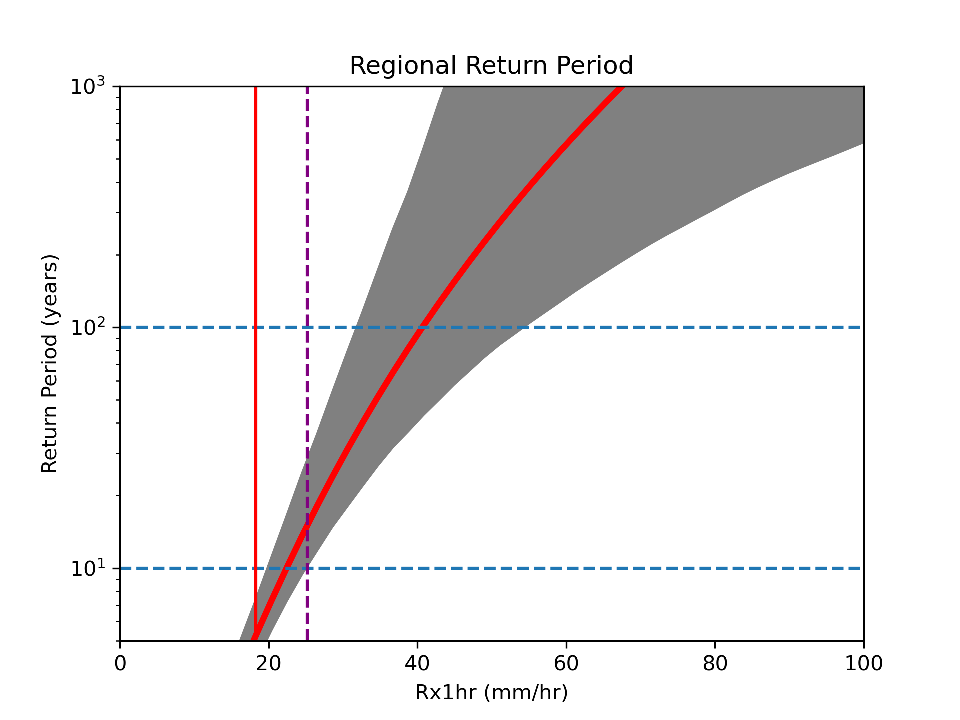
\includegraphics[width=110mm]{radarreturnplot}
    \caption[A line graph plotting the return period in years against the intensity of the event.]{
        A line graph plotting the return period in years against the intensity of the event,
        taken from fitting a GEV distribution to the event distribution.
    The dashed purple vertical line is the intensity of the Stonehaven event.
    The solid red vertical line is the actual one-hour rainfall maximum at the Stonehaven crash location.
    The grey area gives the uncertainties from a Monte Carlo bootstrap of approximately 1000 samples.
    Produced with an adaptation of the code for Figure 2f of~\cite{Tett_Soon}.}
    \label{fig:radarreturnplot}
\end{figure}

It was found that the maximum hourly rainfall at the crash location was 18.2mm/hr and
    that the empirical return period for the Stonehaven event was 17 years,
    as can be seen in Figure~\ref{fig:radarreturnplot}.
The intensity of the Stonehaven event,
    the 0.95 quantile of the radar grid cells having their 2020 seasonal maxima in the AM of the 12th of August,
    was found to be 25.2mm/hr.


\subsection{Model Data}\label{subsec:modelcorr}

\subsubsection{Model Correlations}

\begin{figure}[H]
    \centering
    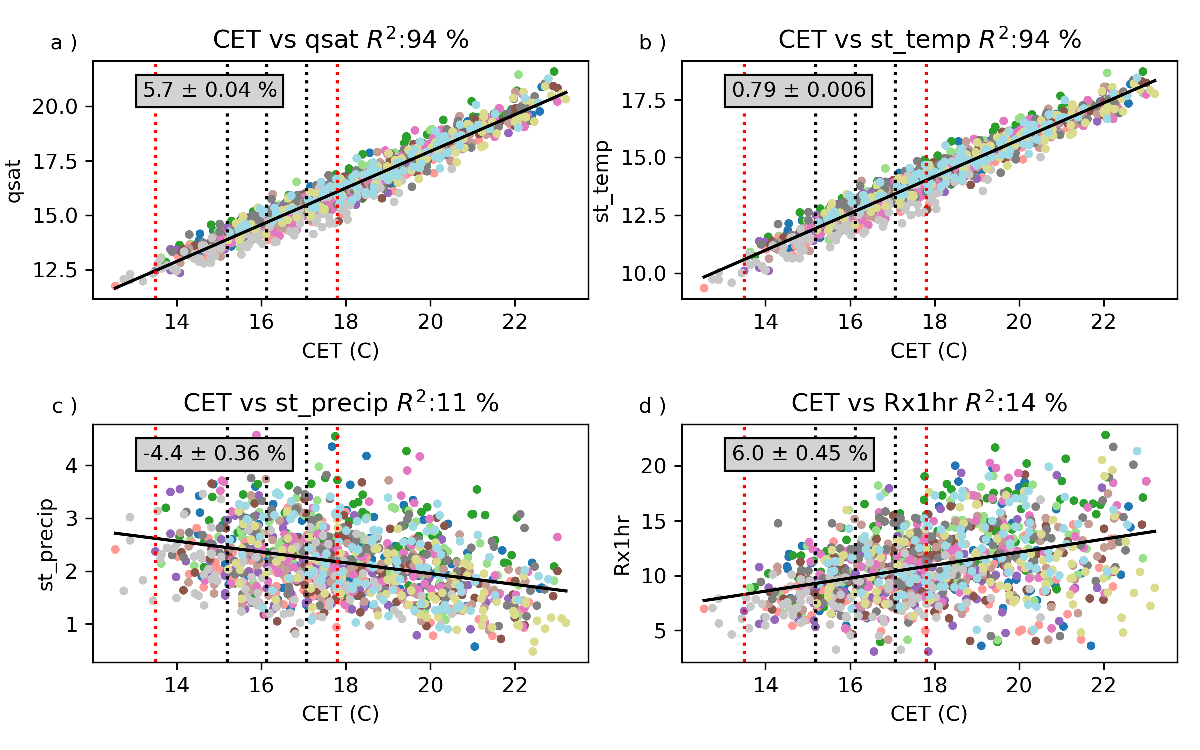
\includegraphics[width=150mm]{2cet_scatter}
    \caption[Scatter diagrams from the Convection Permitting Model.]{
        Scatter diagrams, from the Convection Permitting Model,
        for summer CET vs Stonehaven region saturated humidity (g/Kg) (a),
        Regional Temperature (b),
        Regional  Precipitation (mm/day) (c) and
        spatial median Rx1hr (mm/hr) for the region.
    The region is all points within a square of about 100x100km centred on the Stonehaven crash location.
    Colours indicate the ensemble number, black line is the best-fit regression slope.
    Text box shows best estimate and standard error in the estimated regression.
    Dotted black vertical lines show (left to right) CET summer mean for 1850--1899, 2021 and estimated CET at +2K warming.
    Title shows $R^2$ correlation coefficients for fit.
    Dotted vertical red lines show minimum and maximum CET values from 1850--2020 observations.
    Produced with an adaptation of the code for figure S1 of~\cite{Tett_Soon}}
    \label{fig:2cet_scatter}
\end{figure}

It is unsurprising that the correlations found in (a) and (b) are very similar,
    with both having $R^2$ values that round to the same number to the nearest percentage.
Some data points appear in almost identical points in both scatter diagrams.
This is evident from equation~\ref{eq:qsat}.
By differentiating at $T=18$,
    equation~\ref{eq:qsat} has a Taylor series to first order of $20.5627+1.2863(T-18)$.
By substituting $T=14$ and $T=22$ into this linear approximation,
    only small errors of $0.532$ and $0.603$ are found.
This suggests that in the CET range, equation~\ref{eq:qsat} is effectively linear and so the fit onto the Stonehaven Region saturated humidity
    is a linear scaling of the fit onto the Stonehaven Region Temperature.

(b) finds that the temperature in the Stonehaven Region is expected to increase by 0.79 degrees for every increase
    in CET .
This is of interest, as CET itself is expected to increase by 0.96 per degree of climate warming~\cite{Tett_Soon},
    so the Stonehaven Region temperature is expected to increase far slower than global temperatures.

In (c),
    a negative correlation is found between the mean rain in the Stonehaven region and CET,
    suggesting that total rainfall decreases with an increase in temperature.
This contrasts with the positive correlation between the mean monthly maximum rainfall found in (d),
    which suggests that the scaling of the extreme distribution will be positive.

\subsubsection{Model GEV fit}

\begin{figure}[H]
    \centering
    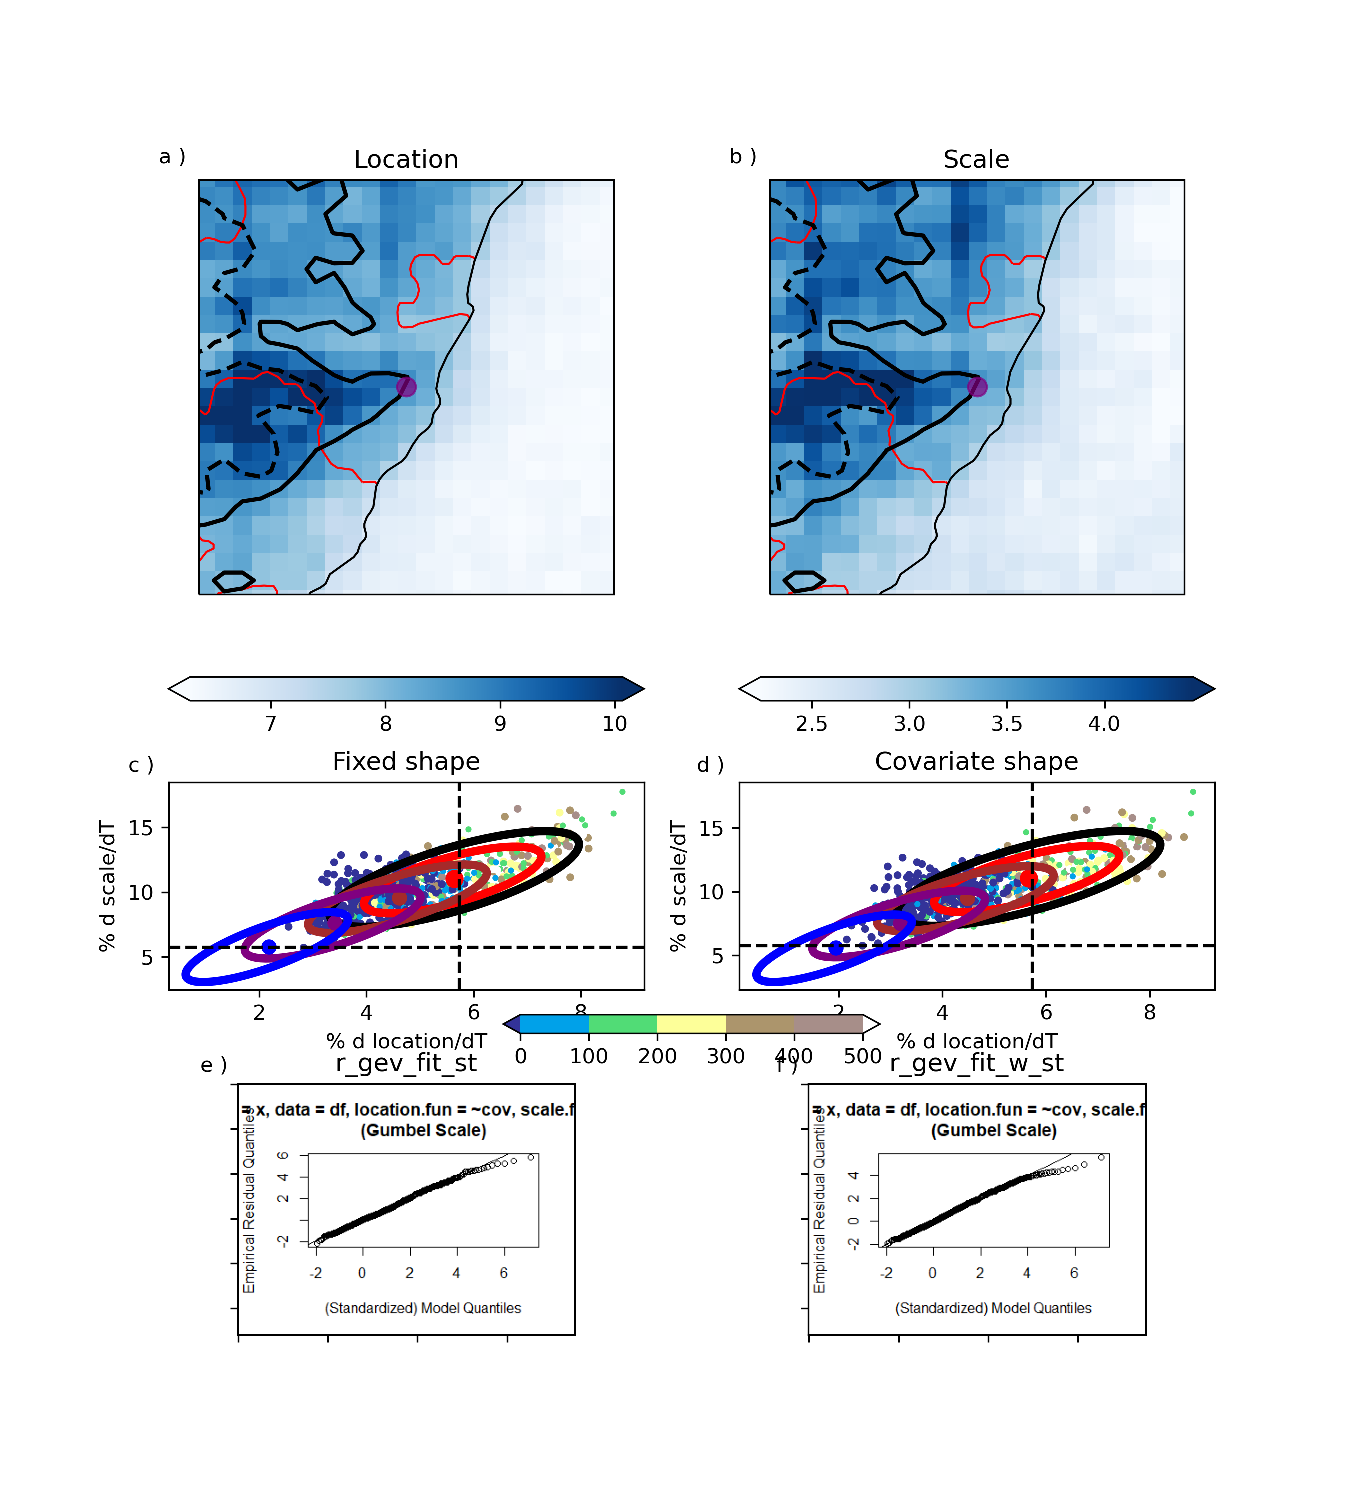
\includegraphics[width=100mm]{2cpm_gev_fit}
    \caption[a) Location parameter $\mu = \mu_0 + \overline{T_{2012-2021}}\mu_1$  for 2012--2021 CET and Rx1hr.
    b) Scale parameter $\sigma = \sigma_0 + \overline{T_{2012-2021}}\sigma_1$ for 2012--2021 CET and Rx1hr.
    c) Scatter plot of d(location)/d(CET) vs d(scale)/d(CET) as of 2012--2021 parameters.
    d) as c) but for case with shape parameter varying with CET.
    e) QQ-plot for GEV fit to CPM data using CET as a covariate at the Stonehaven Crash location.
    f) as e) but for point 25km west of the Stonehaven Crash Location.]{
        a) Location parameter $\mu = \mu_0 + \overline{T_{2012-2021}}\mu_1$  for 2012--2021 CET and Rx1hr.
    b) Scale parameter $\sigma = \sigma_0 + \overline{T_{2012-2021}}\sigma_1$ for 2012--2021 CET and Rx1hr.
    c) Scatter plot of d(location)/d(CET) vs d(scale)/d(CET) as of 2012--2021 parameters.
    Dashed lines show expected changes if changes predicted by Clausius-Clapeyron relationship.
    Dots are colored by topography.
    Large red dot shows mean over all points where height is more than 0m and less than 400m.
    Red ellipse shows 95\% uncertainty for this mean, see subsection~\ref{subsec:riskratios}.
    Other colored large dots and ellipses show similar means and uncertainty ellipses for Rx2hr (brown), Rx4hr (purple) and Rx8hr (blue).
    Black ellipse shows 95\% uncertainty for all Rx1hr points where height is less than 0m and more than 200m.
    d) as c) but for case with shape parameter varying with CET
    e) QQ-plot for GEV fit to CPM data using CET as a covariate at the Stonehaven Crash location.
    f) as e) but for point 25km west of the Stonehaven Crash Location.
    Produced with an adaptation of the code for figure S3 of~\cite{Tett_Soon}}
    \label{fig:2cpm_gev_fit}
\end{figure}

The thin, thick and dashed lines on (a) and (b) represent 0m, 200m and 400m contours respectively.
These charts show that the rainfall is expected to be greater over higher areas,
    with the extreme rainfall distribution having both greater location and scale parameters,
    which are a factor of approximately 1.5x greater over 400m than they are between 0m and 200m.
The rainfall over the sea is extremely low.
This should be disregarded for reasons given in subsection~\ref{subsec:preprocess}

The colours of the dots in (c) show that the increase of both the shape and scale parameters with CET
    increases with height,
    although, as a proportion of the base parameter, there is no evidence for additional scaling with height,
    as, from (a) and (b), higher grid cells have higher base values for the parameters.
The confidence ellipses show that there is far greater uncertainty about the increase in the location parameter
    than the scale parameter.
The similarity of (b) and (c) suggest that fitting the shape parameter as to the covariate does not have
    a significant effect on the fit of the other two parameters to the covariate.
Table~\ref{tab:CCtable} gives the location of the red, brown, purple and blue dots relative to the
    dashed lines representing Clausius-Clapeyron scaling.

(e) shows that the quantiles for the GEV fit are similar at the Stonehaven Crash location,
    while (f) is taken from a point near the 400m contour.
At this point, the GEV fit breaks down at the top end,
    with the GEV fit expecting values far greater than those provided by the CPM model it is fit to.

\begin{table}[H]
    \centering
    \begin{tabular}{c c c c c}
        Covariate\textbackslash Data & Rx1h & Rx2h & Rx4h & Rx8h \\
        None &7498&6533&5341&4130 \\
        CET &7433&6482&5305&4109 \\
        CET w/ Shape &7434&6483&5305&4109 \\
        CPM Region &7402&6457&5287&4097 \\
        CPM Region w/ Shape &7403&6458&5287&4097 \\
        Stonehaven Region &7402&6457&5287&4098 \\
        Stonehaven Region w/ Shape &7403&6458&5288&4098 \\
        Stonehaven Humidity &7405&6459&5289&4099 \\
        Stonehaven Humidity w/ Shape &7406&6460&5290&4100 \\
    \end{tabular}
    \caption[AIC for maximum summer rainfall]{
        AIC for maximum summer 1, 2, 4 and 8 hourly summer maximum rainfall
        above 0m and below 400m in the Stonehaven Region (+/- 0.5 degrees of the Stonehaven Crash location)
        GEV fits with different covariates.
    The covariates are CET, the average temperature in the CPM region (UK),
    the average temperature in the Stonehaven Region and
    the Saturation Humidity in the Stonehaven Region}
    \label{tab:AICtable}
\end{table}

The values of AIC for different rain intervals are not directly comparable,
    as the fit is to different datasets.
For all covariates,
    it is found that fitting the shape to the covariate had no significant effect on the goodness of the GEV fit.
For the 1-hour maxima,
    fitting the GEV with the CPM Region temperature, Stonehaven Region Temperature and Stonehaven Region Humidity gave almost equally good fits.
It was expected that the fit to the Stonehaven Region Temperature and Humidity would be similar for
    reasons given in the discussion of~\ref{fig:2cet_scatter},
    although Humidity does perform slightly worse as a covariate.
Having no covariate provides a worse fit for the data.

The probability of information loss formula, equation~\ref{eq:AIC_Info},
    can be applied to the AIC values in Table~\ref{tab:AICtable} for the one-hour maximum model rainfall.
This finds that a fit to CET is of order $10^{-7}$ times as probable to be a better fit than to another covariate,
    and that a fit to no covariate is of order $10^{-21}$ times as probable to be a better fit than to a covariate other than CET .

\begin{table}[H]
    \centering
    \begin{tabular}{c c c}
        Dataset\textbackslash Parameter  & Location $\mu$ & Scale $\sigma$ \\
        Rx1hr &0.98&1.92 \\
        Rx2hr &0.80&1.67 \\
        Rx4hr &0.59&1.33 \\
        Rx8hr &0.38&1.01 \\
    \end{tabular}
    \caption[Ratio of mean parameter scalings to Clausius-Clapeyron scaling.]{
        Ratio of mean parameter scalings to Clausius-Clapeyron scaling, $\left( \frac{\alpha_1}{\alpha_0} \right) / \left( \frac{H_1}{H_0} \right)$,
        for parameter $\alpha$ in the GEV fit to CET and saturated humidity $H$ in a linear fit to CET,
        where the shape parameter is fixed for the fit.
        Subscript $0$ is the value in the average summer CET of 2012--2021,
            subscript $1$ is the increase for every degree increase of CET.
    Clausius-Clapeyron scaling is 5.73\%.}
    \label{tab:CCtable}
\end{table}

The scalings of all the parameters in Table~\ref{tab:CCtable} are positive,
    as would be expected from Figure~\ref{fig:2cet_scatter} (d),
    which shows that the maximum rainfall extrema increase with CET .
For the one-hour rainfall maxima,
    the location is scaled almost exactly as would be expected with Clausius-Clapeyron,
    shown by the red dot in Figure~\ref{fig:2cpm_gev_fit} (c) being almost exactly on the vertical dashed line,
    while the scale parameter is scaled almost double that expected by Clausius-Clapeyron.
Figure~\ref{fig:2cet_scatter} (a) and (d) also suggest this pattern,
    as both the saturated humidity and 1-hour maximum rainfall increase by around 6 (ignoring units)
    per degree increase in CET, while saturated humidity takes a value at around 15 for a typical CET,
    with Rx1hr taking a value of 10 and so having a larger proportional increase per degree of warming.
This agrees with the IPCC working group 1 assessment~\cite{IPCC_2021},
    finding that sub-daily extreme precipitation scales between one and two times that of Clausius-Clapeyron.

As the time period of the extrema increases,
    the scalings of the parameters decrease.
Figure~\ref{fig:2cet_scatter} (c) suggests that this is to be expected,
    as non-extreme rainfall in the Stonehaven decreases with CET and so by averaging over a longer time period,
    the maximum rainfall exhibits behaviour more similar to average rainfall.
However, this finding is surprising in a wider context,
    as the IPCC assessment~\cite{IPCC_2021} states that scaling in excess of Clausius-Clapeyron should apply to all sub-daily precipitation extremes,
    and all of the extrema given in this report are sub-daily.

The scale parameter $\sigma$ scales by more per increase in CET than the location parameter $\mu$.
The effect of this is that the modelled maximum rainfall in a typical year does not increase by a large amount,
    but for more extreme years, those with higher return periods,
    the maximum rainfall increases by a larger amount with CET than would be expected with Clausius-Clapeyron.

Where the shape parameter is fit as a covariate,
    the change in the shape parameter per degree increase of CET $\xi_1$ is
    0.004, 0.055, 0.128 and 0.252 for the maximum summer model rainfall in
    1 hour, 2 hour, 4 hour and 8 hour time periods respectively.
The risk ratios will be calculated using the one-hour maximum,
    so the covariate fit of the shape parameter is expected to have little effect on these.

\subsection{Risk Ratios}\label{subsec:riskratio}

\begin{figure}[H]
    \centering
    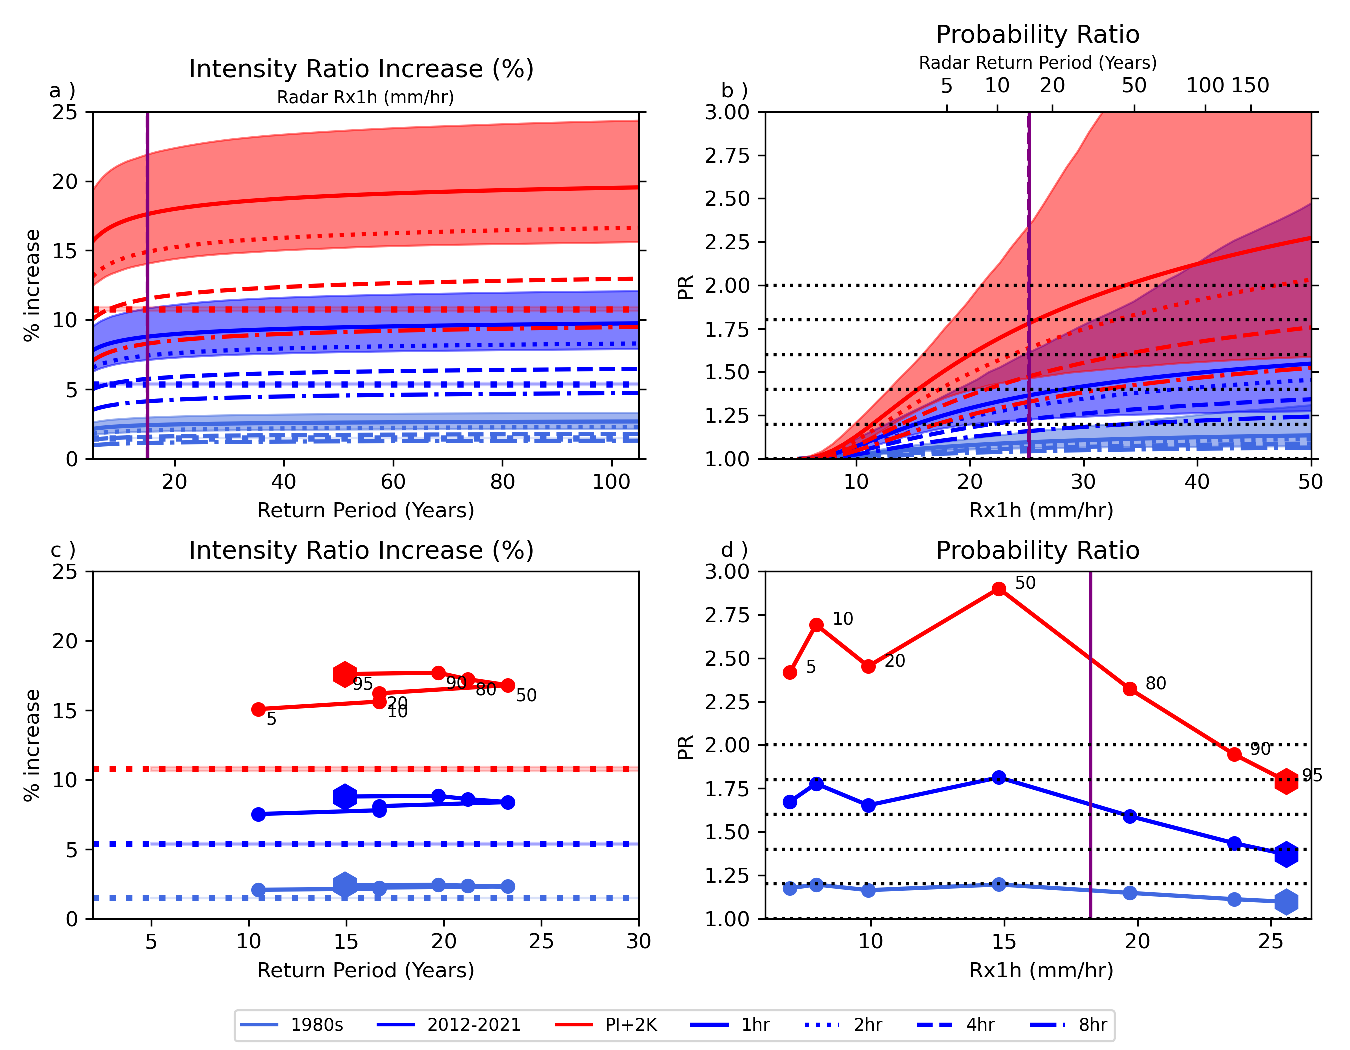
\includegraphics[width=\linewidth]{2probradarcpm}
    \caption[Intensity ratio (\%) as a function of the return period (a,c) and
    probability ratio as a function of regional Rx1hr (b, d).
    ]{
        Intensity ratio (\%) as a function of the return period (a) and
    probability ratio as a function of regional Rx1hr (b).
    The best estimate (line) and 5--95\% uncertainty range (shading) are shown.
    Horizontal dotted lines in a) show expected intensity change if extremes scale with Clausius-Clapeyron.
    The top axis in a and b shows the equivalent rainfall and return period estimated from the radar rainfall data while
    vertical purple line shows the regional rainfall maximum for 2020.
    Dotted, dashed and dot-dashed lines in a and b show results when scaling estimated from simulated 2, 4 and 8 hourly summer maxima (Rx2hr, Rx4hr and Rx8hr).
    c) Intensity ratio (\%) as a function of return period for best estimates using different quantiles (labels on PI+2K line) to define regional extreme.
    Hexagon markers show 95\% quantile used in a and b.
    d) As c) but for probability ratio as a function of Rx1hr.
    Vertical purple line shows Stonehaven Crash Rx1hr for 2020-08-12.
    Note these are different from the regional 95\% quantiles shown in (a) and (b).
    Produced with an adaptation of the code for Figure 3 of~\cite{Tett_Soon}.}
    \label{fig:2probradarcpm}
\end{figure}

Figure~\ref{fig:2probradarcpm} (a) shows that the intensity ratio decreases when fitted to model extrema over longer intervals,
    only being sub-Clausius-Clapeyron when the event distribution is scaled like the average over 8-hour model maxima;
(b) shows the same decrease in risk ratios for scaling like longer-interval model maxima.
This is to be expected from the data in Table~\ref{tab:CCtable},
    as it is known that maxima over longer periods give a lower scaling.

The intensity and probability ratios in (a) and (b) increase with the return period and event intensity.
This is as short return period/low-intensity events are in the bulk of the GEV distribution
    where the location parameter $\mu$ dominates, while long return period/high-intensity events are in the tail of
    the distribution, where scale parameter $\sigma$ dominates behaviour.
The ratio of the intensity ratio to the Clausius-Clapeyron scaling, given by the dotted lines,
    tends to the scaling of $\sigma$ relative to Clausius-Clapeyron,
    given in table~\ref{tab:CCtable}, multiplied by the CET difference from Pre-Industrial as the return period tends to infinity.
The intensity ratio of the scaling of $\mu$ multiplied by CET difference occurs at a return period of
    $\left( 1- e^{-1} \right)^{-1} \approx 1.6$, obtained by inverting equation~\ref{eq:gevreturn}.

(c) Shows that there is little difference in the intensity ratio by defining the Stonehaven Event by a different
    quantile, with all the intensity ratios super-Clausius-Clapeyron and within the confidence interval
    for the intensity ratio of the 0.95 quantile visible in (a).
(c) also shows that the most unusual extrema of the Stonehaven Event were at the 0.5 and 0.8 quantiles,
    both being rarer than 1-in-20-year events, as opposed to the 0.95 quantile definition used in the
    rest of the analysis, which was a 1-in-17 year event.

(d) shows that the probability ratio decreases with the quantile chosen for event definition from the 0.5 quantile onwards,
    going from the 0.5 quantile having a probability ratio of almost 3,
    while the 0.95 quantile has a probability ratio of around 1.8, visible in from the solid red line (b).
Additionally, (d) shows that the Stonehaven Crash location had maximum rainfall between the 0.5 and 0.8 quantiles of the Stonehaven Event,
    not at the 0.95 quantile.

\begin{figure}[H]
    \centering
    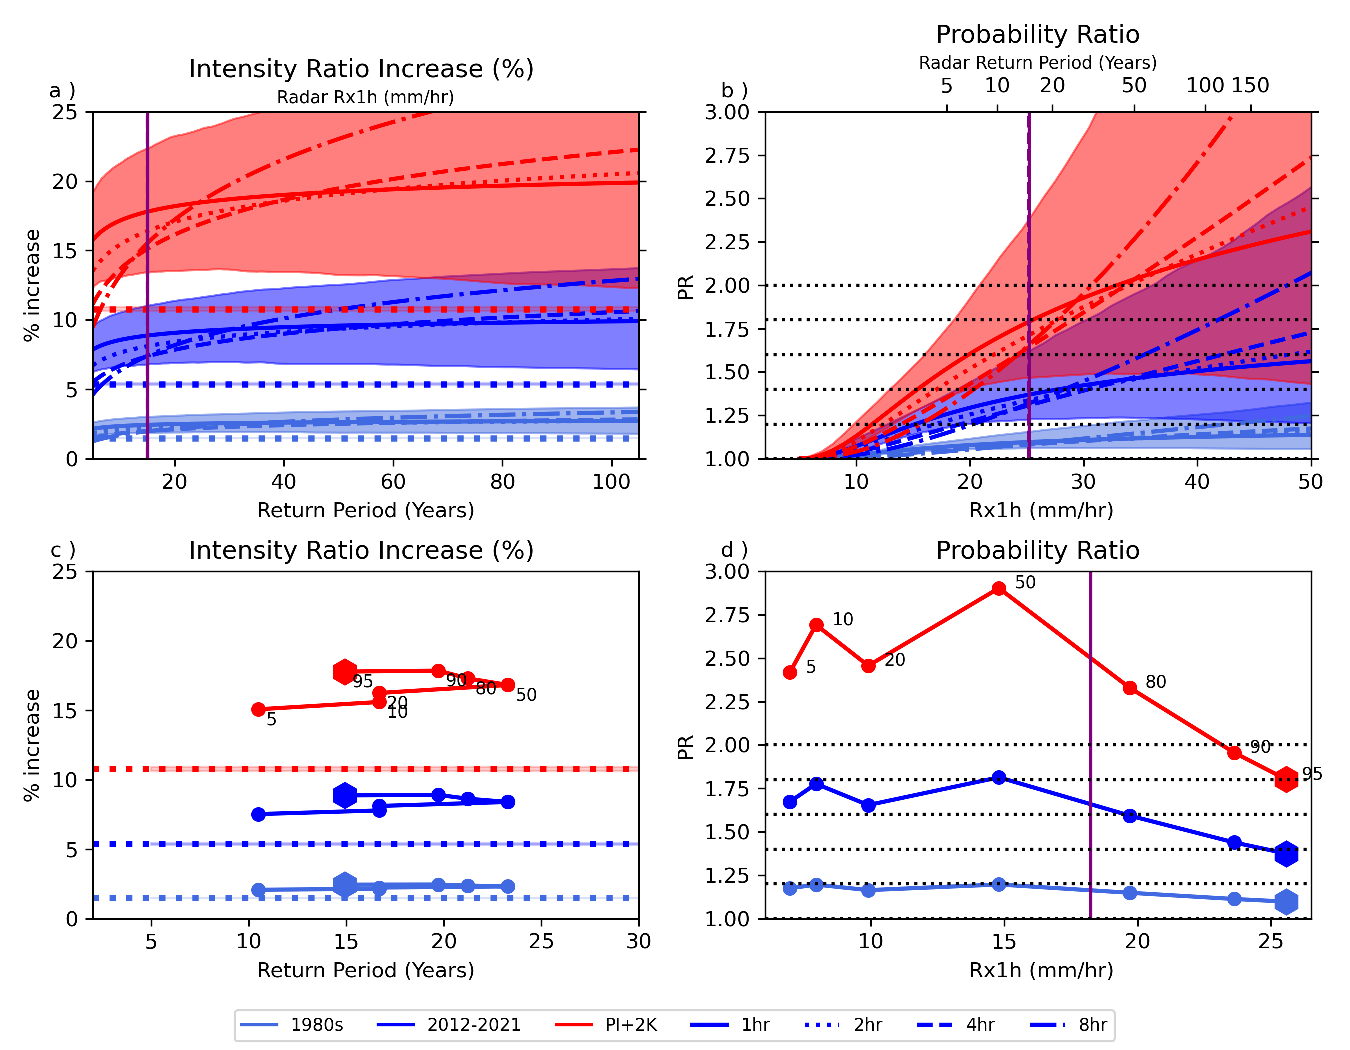
\includegraphics[width=\linewidth]{2probradarcpmshape}
    \caption[Figure~\ref{fig:2probradarcpm} with a covariate fit shape.]{
        As for Figure~\ref{fig:2probradarcpm},
    with the shape parameter also allowed to vary with CET.}
    \label{fig:2probradarcpmshape}
\end{figure}

Figure~\ref{fig:2probradarcpmshape} (c) and (d) show no difference from (c) and (d) of~\ref{fig:2probradarcpm}.
This allows it to be concluded that fitting the shape parameter of the Rx1hr model data as to a CET covariate has
    no impact on the intensity or probability ratio,
    independent of the choice of quantile used to define the intensity of an Event.

(a) and (b) show the same effects as (a) and (b) of~\ref{fig:2probradarcpm} at the return period and intensity
    of the Stonehaven Event,
    with the ratios decreasing with the time interval of model maxima fit to,
    except with broader (weaker) confidence intervals.
However,
    for events with a return period of more than 25 years or an intensity of more than 30mm/hr,
    the effect starts to reverse,
    with the fit to the 8-hour model maxima giving the largest ratios.
The pattern in (a) and (b) of Figure~\ref{fig:2probradarcpm} is completely reversed by return periods of
    more than 45 years or intensities of more than 35mm/hr,
    with both the intensity and probability ratios increasing with the time interval of the maxima.
This occurs as the increase in the shape parameter with CET for the larger model maxima time intervals causes the
    distributions scaled to these to also have a larger shape parameter,
    and so a longer tail and greater likelihood of more extreme events.

\begin{table}[H]
   \centering
    \begin{tabular}{c c c}
        Time Period & Intensity Ratio (\%) & 5--95\% Confidence Interval (\%) \\
        1980s & 2 & 2--3 \\
        2012--2021 & 9 & 7--11 \\
        PI+2K & 18 & 14--22 \\
        With varying shape: && \\
        1980s & 2 & 2--3 \\
        2012--2021 & 9 & 7--11 \\
        PI+2K & 18 & 13--22 \\
    \end{tabular}
    \caption[A table with the intensity ratios.]{
        A table with the intensity ratios $I_1/I_0$ for three different time periods,
        both with and without a covariate shape parameter.
    $I_1$ is the intensity of the event in the Time Period.
    $I_0$ is the intensity of the event Pre-Industrial (1850-1899).}
    \label{tab:irtable}
\end{table}

\begin{table}[H]
   \centering
    \begin{tabular}{c c c}
        Time Period & Probability Ratio & 5--95\% confidence interval \\
        1980s & 1.10 & 1.06--1.15 \\
        2012--2021 & 1.37 & 1.22--1.61 \\
        PI+2K & 1.78 & 1.46--2.34 \\
        With varying shape: && \\
        1980s & 1.10 & 1.06--1.15 \\
        2012--2021 & 1.37 & 1.23--1.62 \\
        PI+2K & 1.79 & 1.47--2.38 \\
    \end{tabular}
    \caption[A table with the probability ratios.]{A table with the probability ratios $p_1/p_0$ with confidence intervals for three different time periods,
        both with and without a covariate shape parameter.
    $p_1$ is the probability of the event in the Time Period.
    $p_0$ is the probability of the event Pre-Industrial (1850-1899).}
    \label{tab:prtable}
\end{table}

Tables~\ref{tab:irtable} and~\ref{tab:prtable} show that,
    as expected from the parameters scaling positively with CET,
    both the intensity and probability of the event increase for later time periods,
    when CET is greater.
The ratios represent the intersections of the solid lines with the purple vertical lines in (a) and (b)
    of Figures~\ref{fig:2probradarcpm} and~\ref{fig:2probradarcpmshape},
    with the confidence intervals representing the intersection of the shaded areas with the purple vertical line.

Both the ratios and confidence intervals show either no or very little difference from fitting the shape as a covariate.

By assuming that the Stonehaven event occurred in a month of typical CET to the 2012--2012 time period,
    the change in the intensity from 25.2mm/hr and return period of 17 years can be calculated.
Pre-industrial,
    the event would have had an intensity of 23.1 (CI: 22.7--23.6) mm/hr and a return period
    of 23.3 (20.9--27.5) years.
In a world 2K warmer than industrial,
     the event would have had an intensity of 27.3 (26.8--27.7) mm/hr and a return period
    of 13.1 (11.7--14.2) years.

\begin{table}[H]
    \centering
    \begin{tabular}{c c c}
        Time Period\textbackslash Parameter & Location $\mu$ & Scale $\sigma$ \\
        PI & 10.2 & 3.90 \\
        1980s & 10.4 & 4.02 \\
        2012--2021 & 10.8 & 4.34 \\
        PI+2K & 11.3 & 4.79
    \end{tabular}
    \caption[Parameters of the GEV distribution for the intensity an event.]{
        A table showing the parameters of the GEV distribution for the intensity for an event defined in subsection~\ref{subsec:radarprocess} after
        applying the scaling of the location $\mu$ and scale $\sigma$ parameters to the temperatures of different time periods.}
    \label{tab:0.95params}
\end{table}

The data in Table~\ref{tab:0.95params} does not have the shape scaled from the CET covariate,
    using the fixed shape parameter $\xi = 0.173$ from the empirical fit.
The shape parameter is in the $0.174$--$0.172$ range for all three fits with covariate shape,
    so it effectively duplicates the parameters here.

Note that as the shape parameter is positive,
    this fit suggests that, with an infinite return period, there is no limit on the maximum hourly rainfall.
While is clearly unphysical, the positive shape parameter gives a minimum possible value of event intensity in a given summer as
    -12.3, -12.8, -14.3 and -16.3 mm/hr for the PI, the 1980s, 2012--2021 and PI+2K Time Periods respectively.
This is clearly also unphysical,
    as rainfall cannot be negative,
    showing that the distribution is inappropriate in the infinite limit in either direction.
However,
    the inference is still valid when interpolating in higher probability dense areas of the distribution,
    where the mean event intensity is 13.2, 13.5, 14.2 and 15.0 mm/hr and
    the median event intensity is 11.7, 11.9, 12.4 and 13.1 mm/hr for
    events in the PI, the 1980s, 2012--2021 and PI+2K Time Periods respectively.

\begin{figure}[H]
    \centering
    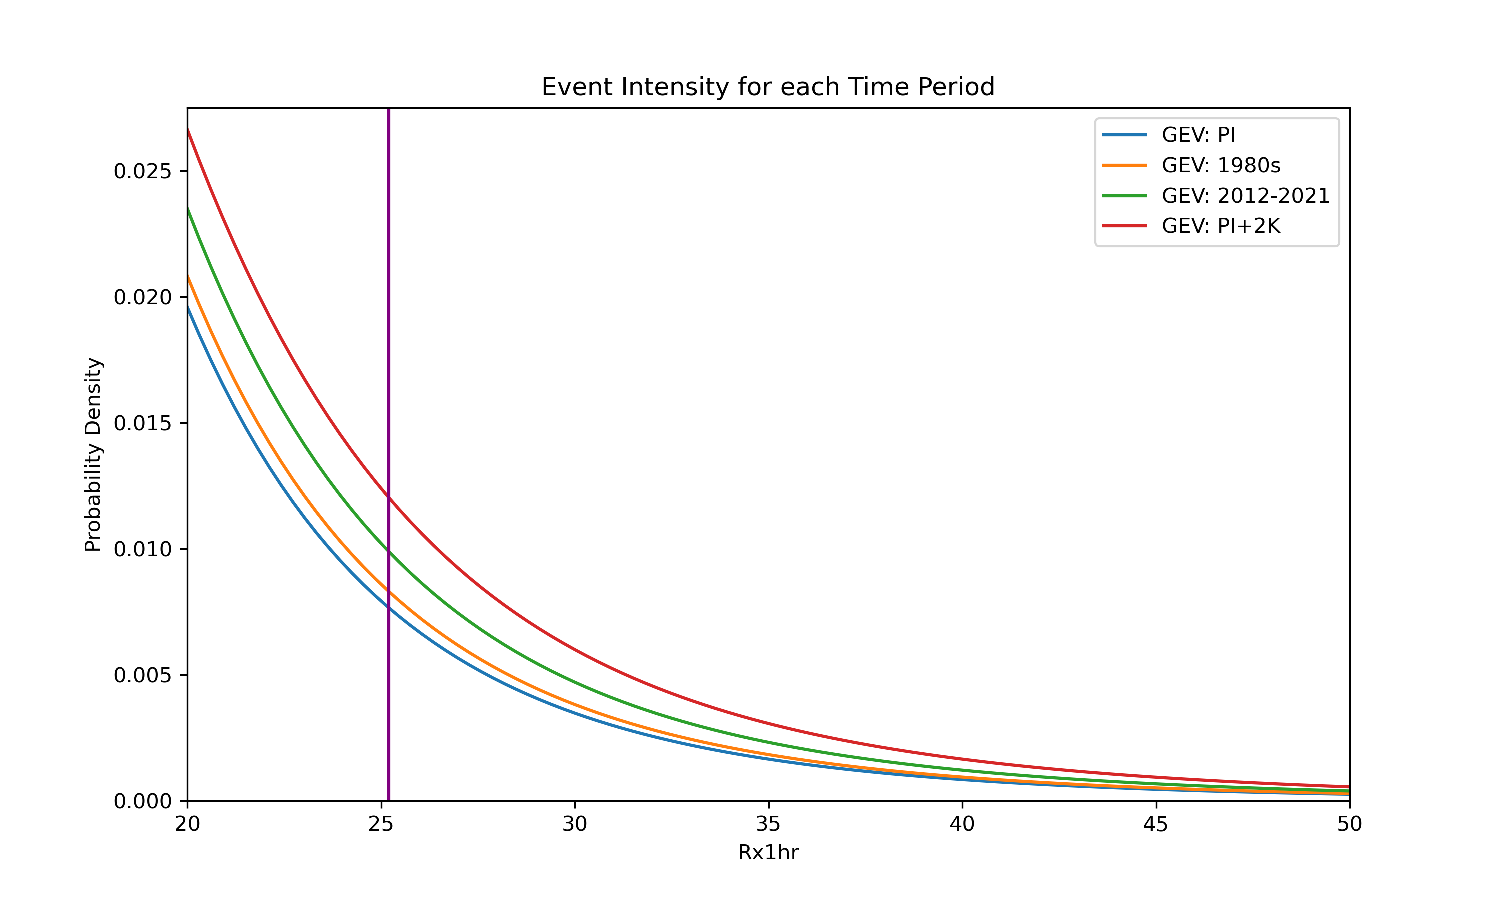
\includegraphics[width=150mm]{scaledgevdists}
    \caption[PDFs of the GEV distributions.]{
        A line chart of the Probability Density Functions of the GEV distributions with parameters given in Table~\ref{tab:0.95params},
        with a shape parameter $\xi = 0.173$.
    The Time periods are Pre-Industrial (PI), the 1980s, 2012--2021
    X-axis gives the 0.95 quantile of the maximum summer rainfall by grid cell in mm/hr,
        Y-axis gives the probability density in probability/(mm/hr).
    Vertical purple line is the intensity of the Stonehaven Event.}
    \label{fig:scaledgevdists}
\end{figure}

Figure~\ref{fig:scaledgevdists} illustrates the probability ratios in the top half of Table~\ref{tab:prtable}.
$p_0$ is the area to the right of the purple line between 0 and the blue curve,
    while $p_1$ is the area to the right of the purple line between 0 and the yellow, green and red curves for
    the 1980s, 2012--2021 and a world 2K warmer than pre-industrial respectively.


\section{Discussion}\label{sec:discussion}

\begin{comment}
This section should give a picture of what you have taken out of your
project and how you can put it into context.

This section should summarise the results obtained, detail conclusions
reached, suggest future work, and changes that you would make if you
repeated the project.
\end{comment}

\subsection{Model Resolution}\label{subsec:dismodeldef}

One difference between the measurement of distributions in the model and the empirical distribution is that the radar data is on a 5x5km grid,
    while the model distributions are fit from model rainfall on a 4.4x4.4km grid constructed from the original 2.2x2.2km model resolution.
Kendon, Fischer and Short~\cite{Kendon_Fischer_Short_2023}, also using 100-year-long 2.2km resolution climate models,
    found that a fine resolution gave a 4x increase in the risk of rainfall exceeding 20mm/hr,
    while a coarser resolution gave only a 2.6x increase.

The model analysis and risk ratio analysis described in section~\ref{sec:model} was repeated,
    except with the model either having no pre-processing other than the height mask,
    maintaining the original 2.2km resolution,
    or with the model being coarsened to take the average of sets of 3x3 grid cells,
    giving a 6.6km resolution.

\subsubsection{Model Fits}

\begin{figure}[H]
    \centering
    \begin{subfigure}{0.48\textwidth}
        \centering
        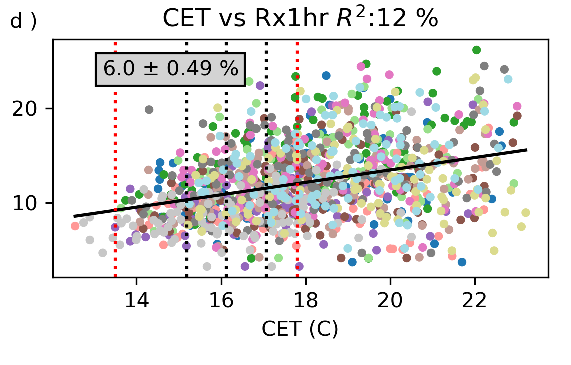
\includegraphics[width=\linewidth]{1cet_scatter}
    \end{subfigure}
    \hfill
    \begin{subfigure}{0.48\textwidth}
        \centering
        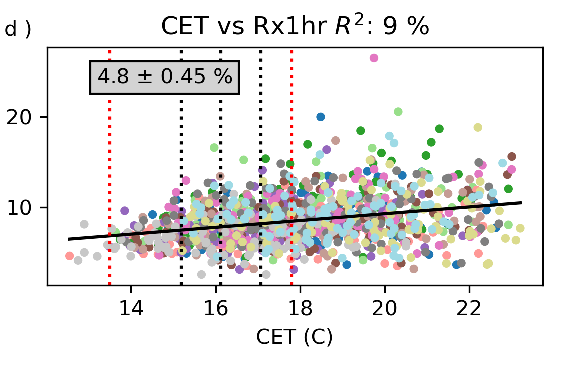
\includegraphics[width=\linewidth]{3cet_scatter}
    \end{subfigure}
    \caption[Figure~\ref{fig:2cet_scatter} with 2.2km and 6.6km fits.]{
        Figure~\ref{fig:2cet_scatter} (d), with the 1-hour model rainfall maxima of the 2.2km resolution (left) and 6.6km resolution (right) models.}
    \label{fig:13cet_scatter}
\end{figure}

Figure~\ref{fig:2cet_scatter} (d) shows that
    one-hour rainfall maxima for the 4.4km model increase by 6.0mm/hr per degree increase in CET,
    matching the increase in the 2.2km model here,
    while the 6.6km model gives a slower increase in rainfall maxima per degree increase in CET .
However, at a typical CET of 16 degrees Celsius,
    the maximum rainfall in the 6.6km is approximately one-fifth smaller than in the other models,
    suggesting that the scaling of the maximum rainfall with CET will be similar.
The 4.4km model is best correlated with CET, with an $R^2$ value of 14\% being greater than either of the alternative models.

\begin{figure}[H]
    \centering
    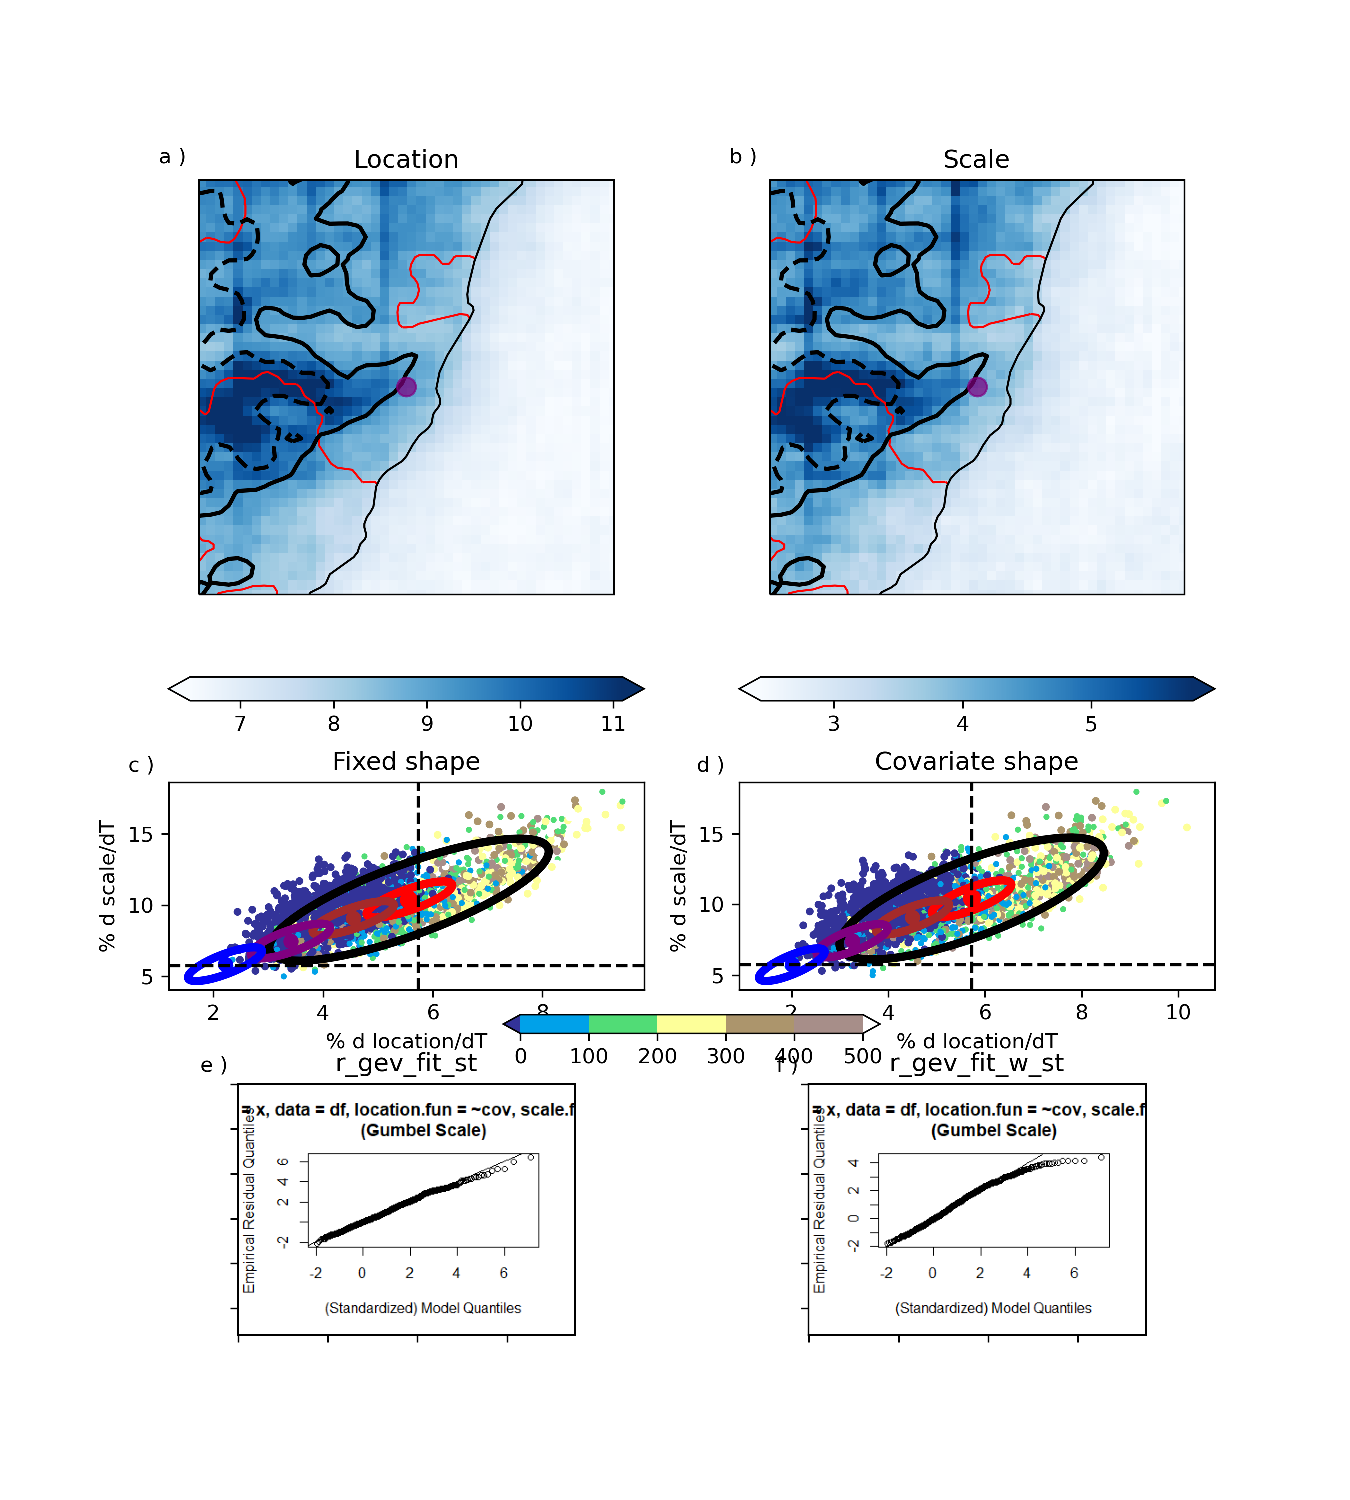
\includegraphics[width=150mm]{1cpm_gev_fit}
    \caption{Figure~\ref{fig:2cpm_gev_fit}, with the 2.2km resolution model}
    \label{fig:1cpm_gev_fit}
\end{figure}

(a) and (b) of figure~\ref{fig:1cpm_gev_fit} appear very similar to
    (a) and (b) of figure~\ref{fig:2cpm_gev_fit}.
However, note that the scale bar is different in each figure,
    with the values being approximately 1.5x greater in the model without coarsening.
This is because the grid cells take maximum summer rainfall values at different times,
    resulting in coarsening before taking the maxima giving results lower than taking the maxima and coarsening after.

(c) and (d) are also very similar between figures~\ref{fig:1cpm_gev_fit} and~\ref{fig:2cpm_gev_fit},
    with the primary difference between them being the smaller (stronger) confidence intervals in the more fine model.
This is to be expected, as there are more data points to be sampled.

\subsubsection{Risk Ratios}

\begin{figure}[H]
    \centering
    \begin{subfigure}{0.48\textwidth}
        \centering
        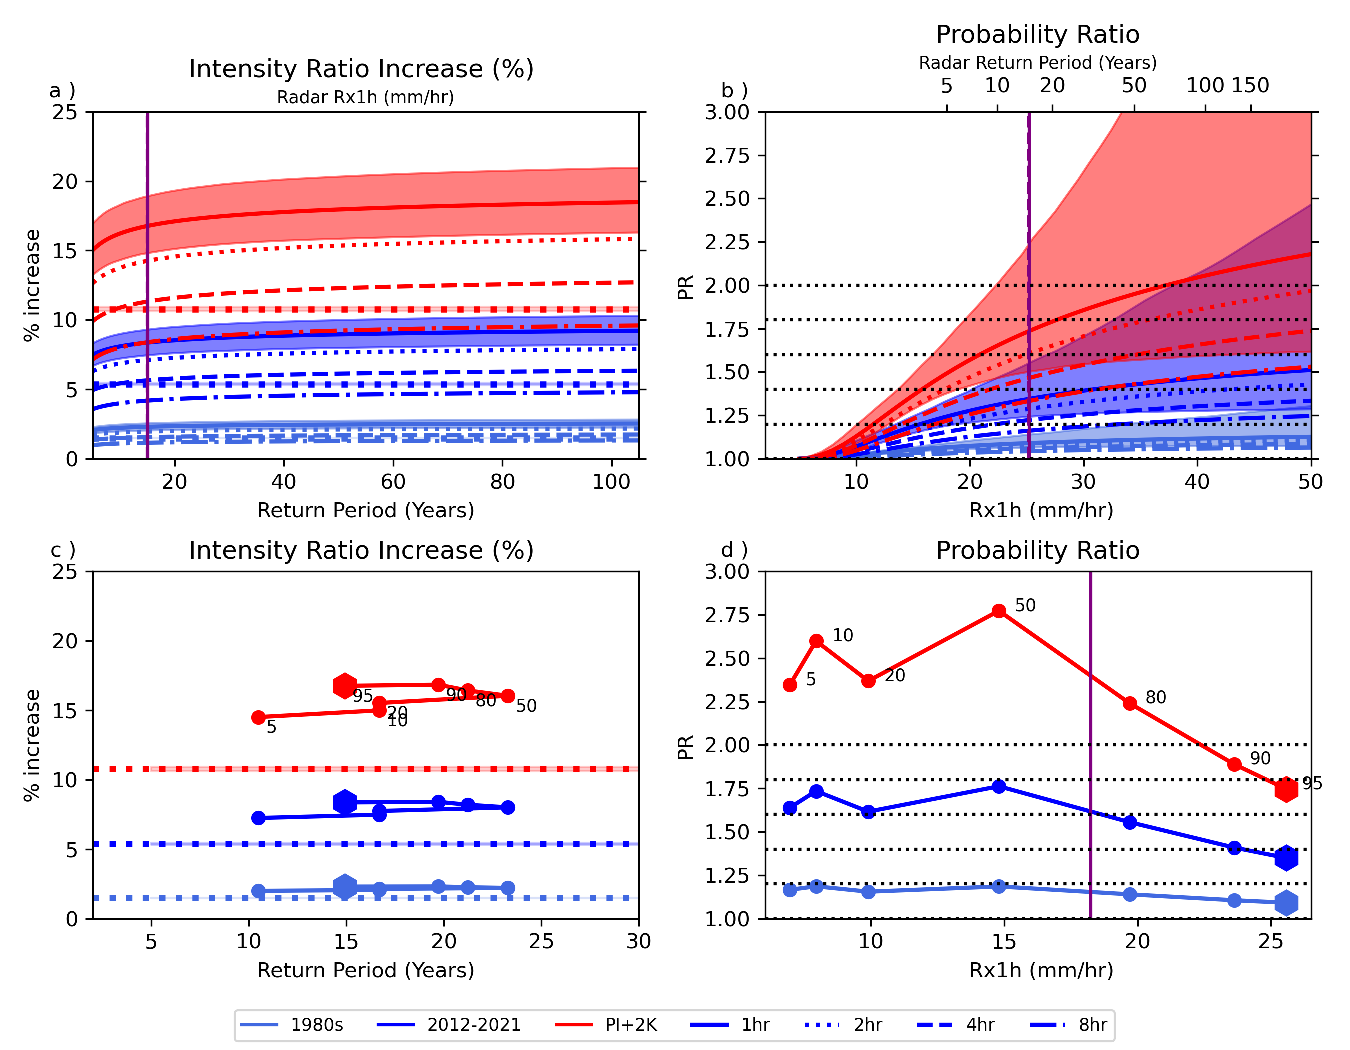
\includegraphics[width=\linewidth]{1probradarcpm}
    \end{subfigure}
    \hfill
    \begin{subfigure}{0.48\textwidth}
        \centering
        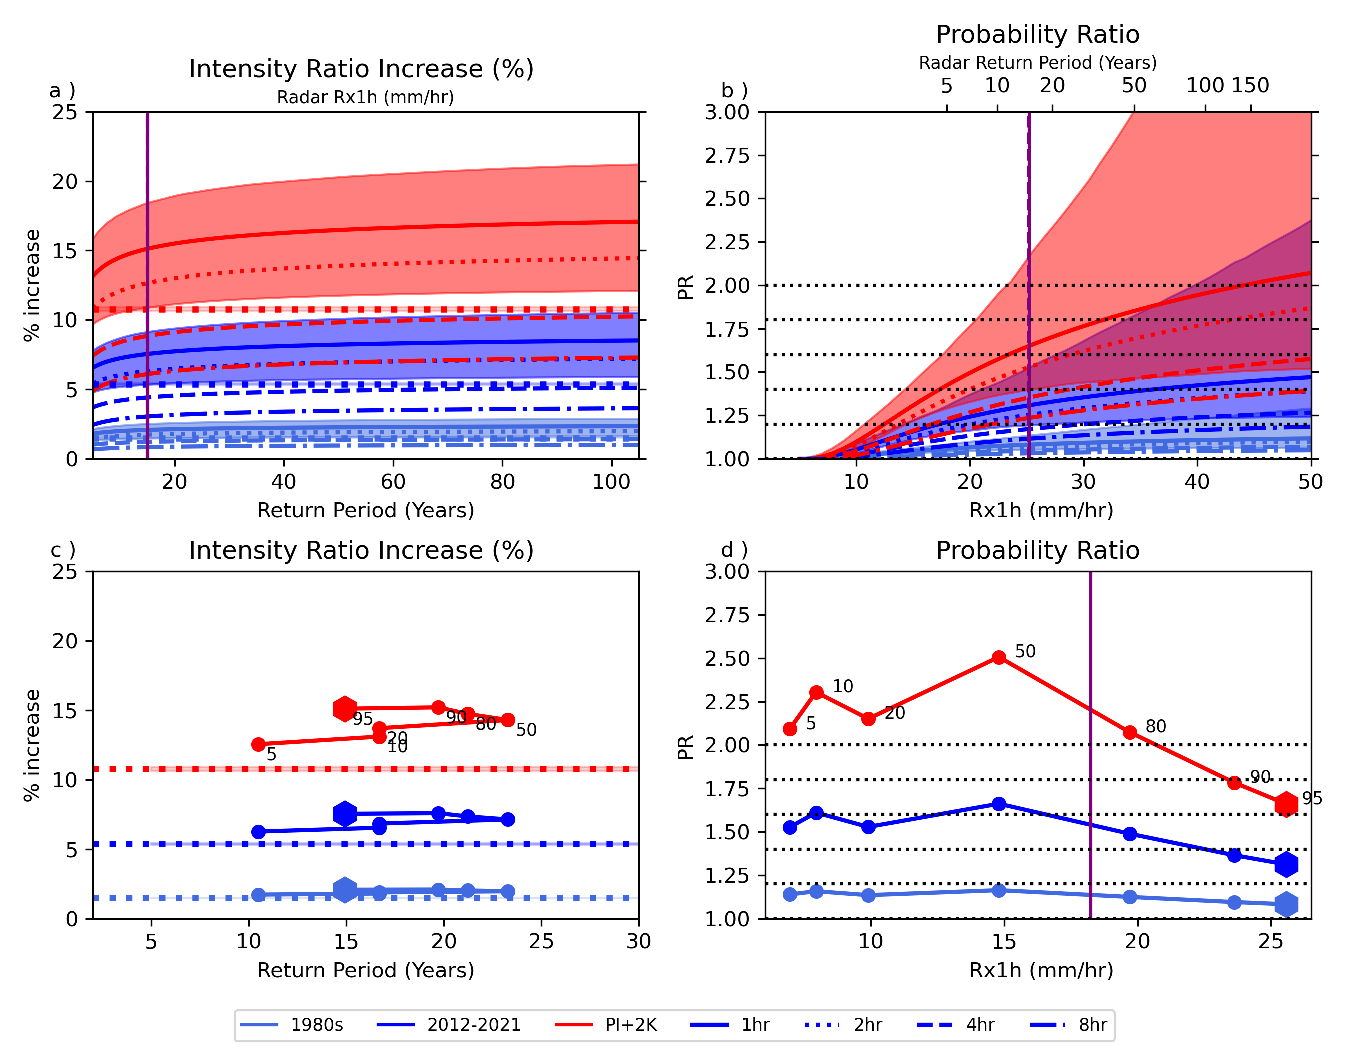
\includegraphics[width=\linewidth]{3probradarcpm}
    \end{subfigure}
    \begin{subfigure}{0.48\textwidth}
        \centering
        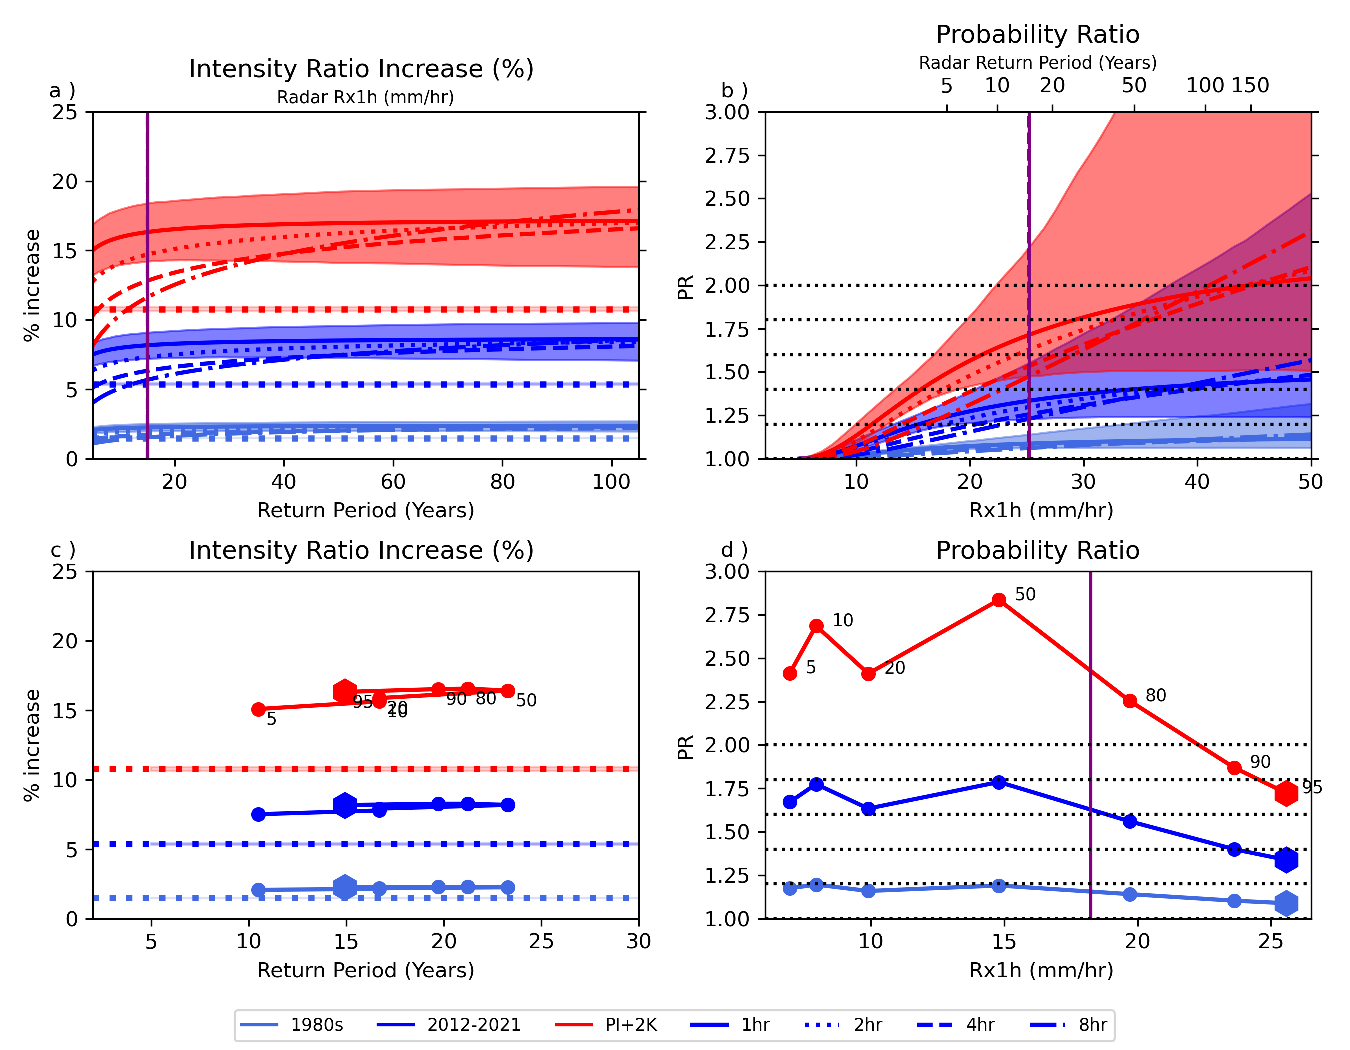
\includegraphics[width=\linewidth]{1probradarcpmshape}
    \end{subfigure}
    \hfill
    \begin{subfigure}{0.48\textwidth}
        \centering
        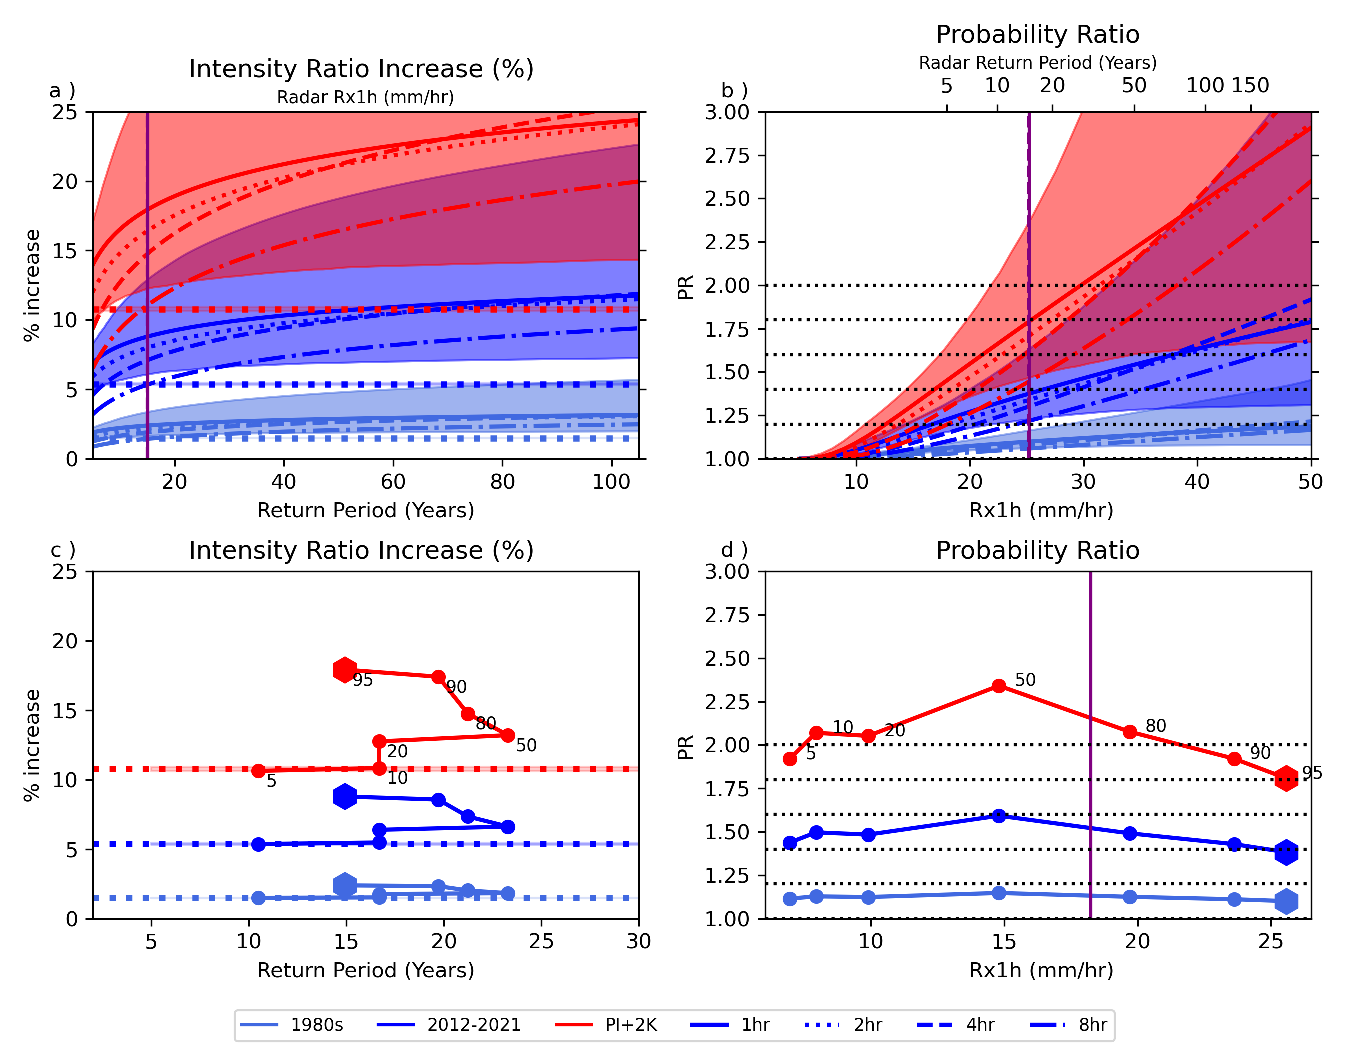
\includegraphics[width=\linewidth]{3probradarcpmshape}
    \end{subfigure}
    \caption[Figures~\ref{fig:2probradarcpm} and~\ref{fig:2probradarcpmshape} for the 2.2km and 6.6km models.]{
        Figure~\ref{fig:2probradarcpm} for the 2.2km model (top left) and the 6.6km model (top right).
    Figure~\ref{fig:2probradarcpmshape} for the 2.2km model (bottom left) and the 6.6km model (bottom right)}
    \label{fig:13probradarcpm}
\end{figure}

One clear difference between the plots in Figure~\ref{fig:13probradarcpm} is the finer confidence intervals
    when working with the 2.2km radar data, due to the dataset being larger,
    as well as the very wide confidence intervals for the 6.6km data,
    due to the lack of data giving poor confidence intervals for the model parameter scalings.

For the ratios obtained from both the 2.2km and 6.6km model,
    similar behaviour to that of the 4.4km is found when looking at the effect of using scalings from model rainfall maximum time intervals larger than 1 hour.
As in Figures~\ref{fig:2probradarcpm} and~\ref{fig:2probradarcpmshape},
    the probability ratio decreases as the time interval decreases where the scale parameter is fixed,
    while when the scale parameter is fit to the CET covariate,
    this only holds up to a point where the relation inverts.
This inversion point seems to be approximately one in 25-year or 35mm/hr events,
    although this does not apply to the 8-hour time interval for the 6.6km fit.

\begin{table}[H]
   \centering
    \begin{tabular}{c c c c c}
        Time Period & IR (2.2km) (\%) & 5--95\% CI (\%) & IR (6.6km) (\%) & 5--95\% CI (\%) \\
        1980s & 2 & 2--3 & 2 & 1--3 \\
        2012--2021 & 8 & 7--9 & 8 & 5--9 \\
        PI+2K & 17 & 15--19 & 15 & 11--18 \\
        With varying shape: &&&& \\
        1980s & 2 & 2--3 & 2 & 2--3 \\
        2012--2021 & 9 & 7--9 & 9 & 6--13 \\
        PI+2K & 16 & 14--18 & 18 & 12--28 \\
    \end{tabular}
    \caption[Table~\ref{tab:irtable} fot 2.2km and 6.6km resolution model fits.]{
        A table with the intensity ratios $I_1/I_0$ for three different time periods,
        both with and without a covariate shape parameter,
        for the 2.2km and 6.6km resolution model fits.
    $I_1$ is the intensity of the event in the Time Period.
    $I_0$ is the intensity of the event Pre-Industrial (1850-1899).}
    \label{tab:13irtable}
\end{table}

\begin{table}[H]
   \centering
    \begin{tabular}{c c c c c}
        Time Period & PR (2.2km) & 5--95\% CI (\%) & PR (6.6km) & 5--95\% CI \\
        1980s & 1.09 & 1.06--1.14 & 1.08 & 1.05--1.13 \\
        2012--2021 & 1.34 & 1.24--1.55 & 1.31 & 1.19--1.52 \\
        PI+2K & 1.74 & 1.50--2.24 & 1.65 & 1.40--2.16 \\
        With varying shape: &&&& \\
        1980s & 1.09 & 1.06--1.14 & 1.10 & 1.06--1.16 \\
        2012--2021 & 1.33 & 1.23--1.55 & 1.37 & 1.23--1.63 \\
        PI+2K & 1.71 & 1.47--2.22 & 1.79 & 1.47--2.36 \\
    \end{tabular}
    \caption[Table~\ref{tab:prtable} for the 2.2km and 6.6km resolution model fits.]{
        A table with the probability ratios $p_1/p_0$ with confidence intervals for three different time periods,
        both with and without a covariate shape parameter.
    $p_1$ is the probability of the event in the Time Period.
    $p_0$ is the probability of the event Pre-Industrial (1850-1899).}
    \label{tab:13prtable}
\end{table}

For the 6.6km resolution data,
    without the shape fit to the covariate,
    the probability ratios suggest that the 4.4km ratios may be an overestimate.
However,
    the ratios match to the nearest hundredth when the shape parameter is fit to the covariate.
As the probability ratios with and without the shape covariate fit are identical for the 4.4km data,
    this suggests that fitting the shape as to the CET covariate may be capturing effects lost from the lower resolution,
    although both of the 6.6km fits have an AIC of 6591, suggesting that it is not likely that any information is lost.
Furthermore, for the 6.6km fit with the shape fit to the covariate,
    the intensity ratios decrease if a quantile lower than 0.95 is chosen to give the intensity of an event.

The intensity and probability ratios from the 2.2km and 6.6km model data in tables~\ref{tab:13irtable} and~\ref{tab:13prtable},
    do not differ significantly from those found from the 4.4km model data in tables~\ref{tab:irtable} and~\ref{tab:prtable},
    as the 4.4km ratios lie in the confidence intervals of both of the alternative models and vice versa.
It can then be concluded that changing the model resolution for gathering the parameter scalings does not have a significant effect
     on the outcomes of the event attribution process.

It would not be expected for this analysis to match the disparity in extreme events found by Kendon, Fischer and Short~\cite{Kendon_Fischer_Short_2023}.
This is as the analysis here applies the parameter scaling from different model resolutions to an already fit empirical distribution,
    while the analysis in~\cite{Kendon_Fischer_Short_2023} measures the probability of the model data crossing a threshold.

The model data resolutions providing similar results suggest that the factors driving the change in the maxima are similar between resolutions.

\subsection{Choices in analysis}\label{subsec:diseventdef}

The analysis in subsection~\ref{subsec:dismodeldef} shows that the choice of a 4.4km model resolution over a finer or coarser resolution
    did not have a significant impact on the results.
However,
    many other choices were made in the analysis.
It is necessary to show that these choices do not have a significant effect on the final outcome for the results to be robust.
Where the choices were found to potentially be impactful,
    it is also useful to state whether a more valid choice would suggest that the results are conservative or overstate the impacts.

\subsubsection{Event Definition}

\begin{itemize} \item Stonehaven Region and height mask \end{itemize}

Defining the Stonehaven Region as a 100km$\times$100km square centred on the crash location was deemed valid,
    as choosing a region based on different factors could potentially lead to bias.
The 0m to 400m height mask was considered a valid choice,
    as the catchment of the drain causing the Stonehaven crash peaked at around 200m,
    making 200m the median point of the rainfall.

Figure~\ref{fig:2cpm_gev_fit} (a) and (b) show that rainfall is much higher in the 200m--400m height range,
    than in the 0m--200m height range
    with Figure~\ref{fig:2cpm_gev_fit} (c) showing that the parameters of the distribution scale more at higher grid cells.
This suggests that the results would understate the risk ratios had a height mask with a lower cap been used.
However, any lower cap would not properly reflect the risk ratios at the Stonehaven crash location,
    as so many points in the 0m--200m height range display far lower rainfall extremes than at Stonehaven.

One additional factor to consider is the homogeneity of the climate of the region used for the analysis.
Looking at the K\"oppen classifications of the Stonehaven Region, given in~\cite{Koppen_file} from WorldClim data~\cite{worldclim},
    the Stonehaven crash location lies on the boundary of Cfb Oceanic and Cfc Subpolar Oceanic.
The difference between these definitions is the average temperature,
    so it is valid to include both.
The height mask prevents the inclusion of the areas classed as Dfc Subarctic and ET Tundra in the Cairngorms National Park
    in the region.

\begin{itemize}\item Time interval of event\end{itemize}

Although, as can be seen from Figure~\ref{fig:stonehavendayraingraph},
    the extreme rainfall at Stonehaven was spread over a four-hour period,
    the event was defined by seasonal one-hour maxima,
    primarily for practical reasons involving the processing of the data.
As this analysis was not done,
    the effect of different time intervals in the definition will be discussed when looking at the effect of
    different time intervals in the model.

\begin{itemize}\item 12-hour bin for event definition\end{itemize}

Each event is defined as occurring within a 12-hour window.
The primary reason for this is to preserve statistical independence,
    as if the seasonal maxima of each grid cell were considered as an extreme rainfall event
    the events may not be independent,
    as extreme rainfall at two locations caused by a single storm would not be independent.

One concern with this approach is that a single storm may pass through the Stonehaven Region
    across two consecutive 12-hour time periods,
    giving two events that are not independent as they describe the same storm.
After applying the minimum size filter discussed in the next bullet point,
    this occurs for 8 of the 77 events,
    which is unlikely to have a significant effect on the validity GEV fit.

The technique used for the fitting of distributions to the model data,
    where each grid cell has a separate distribution fit to the seasonal maxima,
    clearly maintains statistical independence as each maximum occurs in a different year.
This is not possible for the empirical fit as there are only 18 years of seasonal maxima per grid cell,
    as opposed to the 1200 years simulated in the model,
    and only 18 points are insufficient to fit GEV distributions meaningfully without excessively wide confidence intervals.

\begin{itemize}\item Spatial size of event\end{itemize}

\begin{figure}[H]
    \centering
    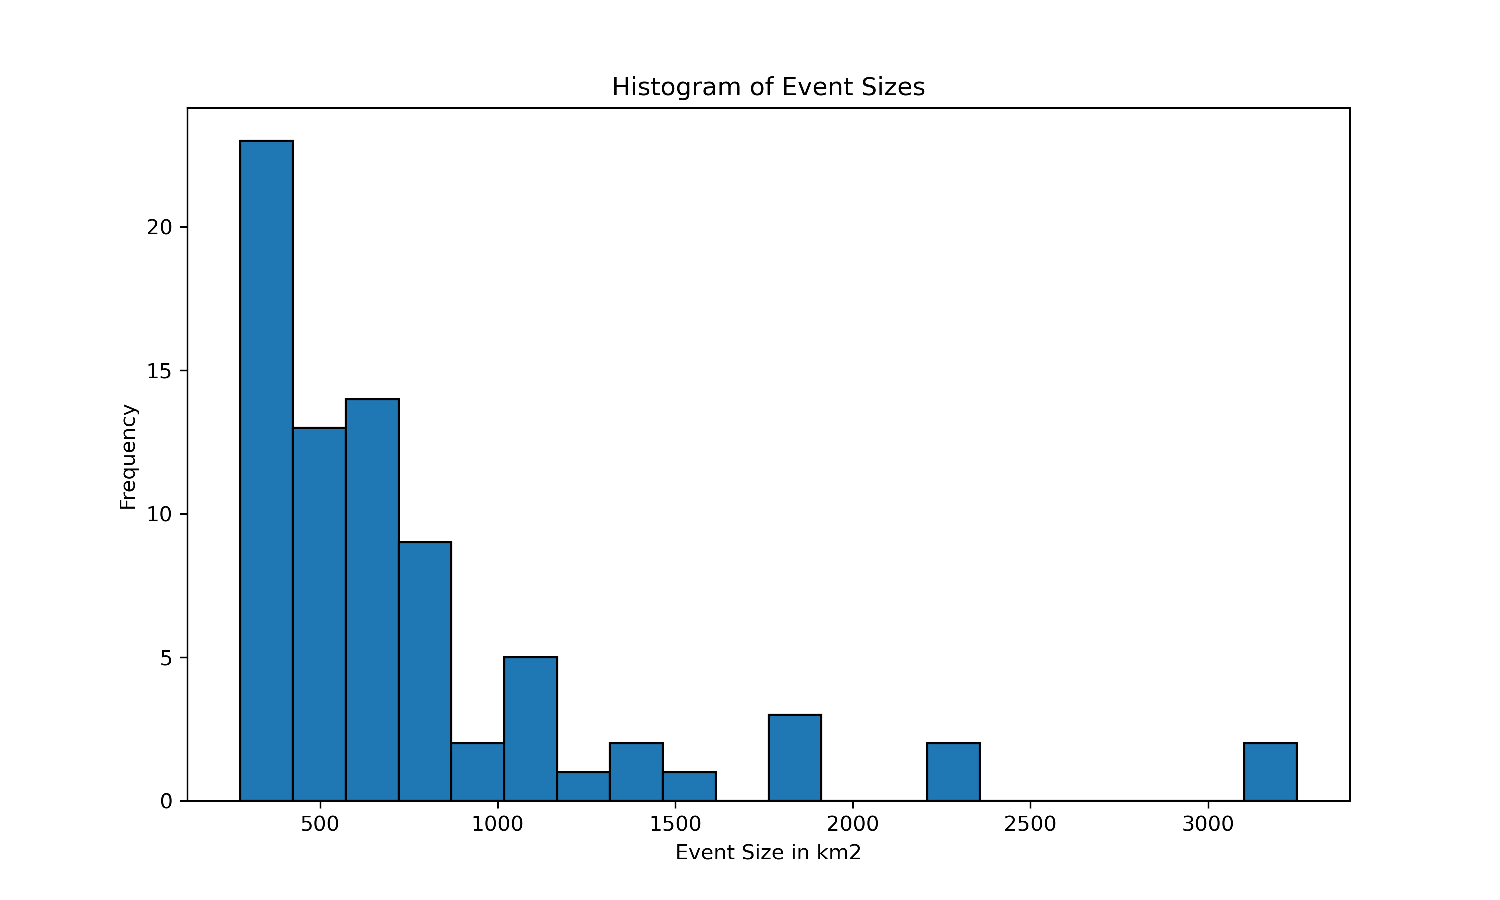
\includegraphics[width=150mm]{eventsizehist}
    \caption[Histogram showing the distribution of event sizes.]{
        Histogram showing the distribution of event sizes in $\text{km}^2$ of the 77 events used to fit the radar data.
    The Stonehaven Event had a size of 3250$\text{km}^2$,
        the event covering the largest amount of space.
    No events lower than 250$\text{km}^2$ are in this histogram as those were removed.}
    \label{fig:eventsizehist}
\end{figure}

Applying the event size filter left only 77 events, as opposed to the 362 separate 12-hour periods in which at least one grid cell had a summer maximum precipitation.
Removing these events was a necessary choice as a single cell reaching a maximum does not represent a summer convective storm similar to that causing the Stonehaven Crash.

However,
    it is clear that there are many events which cover a far smaller area of the Stonehaven Region which are being used in the analysis.
There is only one event covering a similar area,
    occurring on the morning of the 28th of July 2021.
It is interesting that these events both occurred extremely late in the dataset,
    but a sample size of 2 is insufficient to draw any conclusions about the likelihood of these events changing over time or with changes in temperature.

The Stonehaven Event and the 2021 event covered 127 and 130 of the 185 grid cells respectively,
    leaving 2020 and 2021 to have only 1 and 2 events from other grid cells each.
If this is a strong effect on later years,
    then the empirical fit will be biased to earlier years due to all events being weighted equally.
From Figure~\ref{fig:eventsyear}, it can be seen that there is no significant correlation between the
    year and the number of events, so the fit is accurate for the entire time period.

Figure~\ref{fig:eventsyear} provides further evidence that the choice of event size
    was acceptable,
    with the events including the largest 2--7 storms in the region each year.
When a cutoff greater than 250$\text{km}^2$ was imposed,
    one example of which was 500$\text{km}^2$,
    it was possible to find a GEV fit for the whole dataset.
However,
    the Monte Carlo procedure for estimating confidence intervals resulted in many fits
    to random samples with replacement giving significantly anomalous distributions,
    leading to an overall infinite confidence interval.
Figure~\ref{fig:cellsyear} shows the number of cells contributing to events for a given year.
For all years, the majority of the 185 cells are providing data to fit.

\begin{figure}[H]
    \centering
    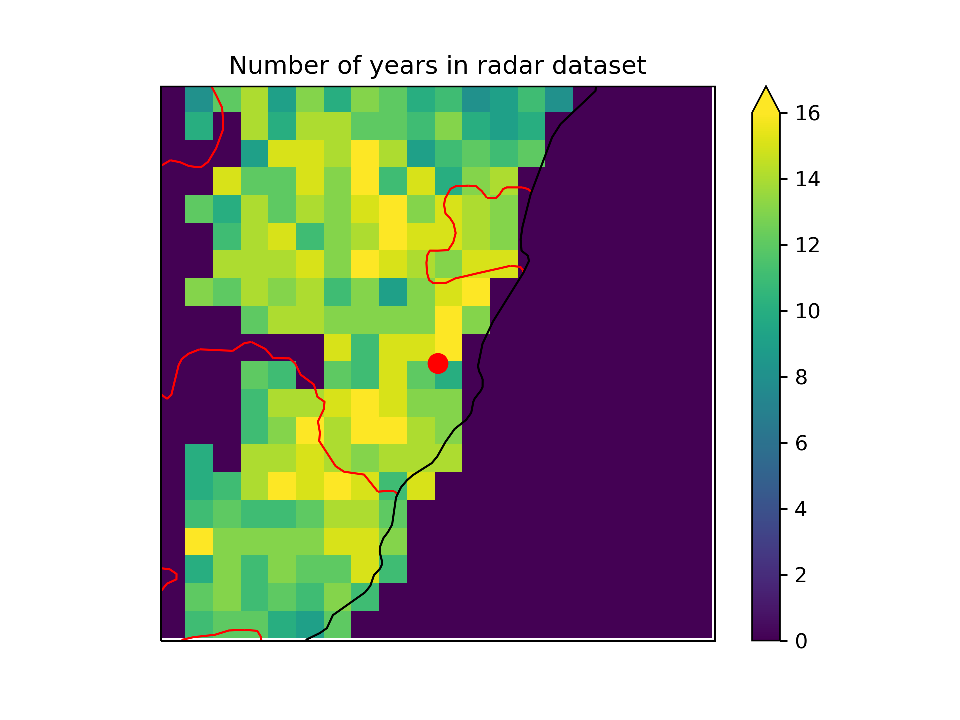
\includegraphics[width=120mm]{yearsinradardata}
    \caption[Plot of the number of years each grid cell appears in an event.]{
        Plot of the number of years each grid cell appears in an event.
    Cells covered by the height mask in Figure~\ref{fig:stonetopogallowed}
        do not provide any data.
    Black lines are coastlines, red lines are local authority boundaries.
    Red dot is the crash location.}
    \label{fig:yearsinradardata}
\end{figure}

Comparing the number of times grid cells provide seasonal rainfall maxima to the set of events
    in Figure~\ref{fig:yearsinradardata} to the topography in Figure~\ref{fig:stonetopog},
    no clear relationship between the topography of the point and the frequency of its appearance in events.
This may suggest that there is no bias towards higher or lower points in the radar data fit.
However,
    as the fit is made to an upper quantile (0.95) of the maximum rainfall at the points contributing to an event,
    this does not directly imply that the fit will not be biased.
For example, if the highest points provide maxima that are in the top quantiles of the event,
    these will have a larger impact on the magnitude used to define the event.

On the other hand,
    by comparing Figure~\ref{fig:yearsinradardata} with Figure~\ref{fig:stoneregionrain},
    it is seen that the locations of Stonehaven Event are represented disproportionately in the
    locations used to draw the sample of events.
This suggests that the results are more specific to the Stonehaven Event than to other extreme rainfall in the region.
It is unsurprising that the grid cells nearer the centre of the region appear in more events,
    as grid cells nearer to the boundary are more likely to take their summer rainfall maxima
    as a part of a storm that passes near the Stonehaven Region but is not sufficiently close to
    result in 10 cells taking a maximum value and qualifying as an event.

\begin{itemize}\item Quantile used for intensity of event\end{itemize}

As noted in the discussion of figure~\ref{fig:2probradarcpm},
    the rainfall at the location of the Stonehaven Crash was between the 0.5 and 0.8 quantiles of the Stonehaven Event,
    and the Stonehaven Event was especially unique with the 0.5 and 0.8 quantiles having larger return periods.
This suggests that one of these quantiles may be a more appropriate definition of the intensity of an event,
    as opposed to the 0.95 quantile used for the analysis.

Figure~\ref{fig:2probradarcpm} (c) shows that the intensity ratio is not significantly changed by a choice of parameters,
    suggesting that the intensity ratios found here are robust,
    while (d) shows that the probability ratio is lower for the 0.95 quantile used in the analysis than either of the alternative quantiles,
    suggesting that the probability ratios found here are conservative,
    underestimating the effect of Anthropogenic Climate Change.
As figures~\ref{fig:2probradarcpmshape} and~\ref{fig:13probradarcpm}
    also exhibit this behaviour,
    both of these findings are themselves robust relative to a change in model resolution or a CET scaling of the shape parameter.

The choice of the 0.95 quantile in the original analysis was valid as this is a `more extreme' quantile and was thought to best capture the event's
    effects on the region, as opposed to at the crash location.
The trend in probability ratios continuing for all 4 of the quantiles $\geq$ 0.5 shows that an actual effect is occurring,
    as opposed to an artefact of the 0.95 quantile potentially being ill-defined for small events where fewer than 20 grid cells take seasonal maxima.

\subsubsection{Model Fit}
\begin{itemize}\item Use of different definition from radar data\end{itemize}

As noted in the discussion of 12-hour bins,
    the fit to the model is taken to be the average over the parameters for each grid cell,
    as opposed to the fit to the empirical data being to events as defined above.
For the application of the scaling from the model to be valid,
     it is necessary to justify that the parameters of the event distribution should scale with
    the average parameters of seasonal maximum rainfall of a grid cell in the model.

Each event intensity is,
    by taking a 0.95 quantile,
    effectively a median average over the set of grid cells with seasonal maximum rainfall in the top decile of an event.
It is clear that this would result in both parameters being larger compared to a distribution of seasonal maxima at a single cell,
    as the cells with the largest maximum rainfall are taken to define the distribution.
This is not a concern,
    as the parameter scalings are multiplicative and so proportional to the size of the parameter being scaled,
    seen in equation~\ref{eq:newradarparams}.

However,
    it is uncertain whether this would result in a change in variability between the distributions.
As the event intensity is,
    an effective average over the maximum of multiple grid cells,
    this suggests that there would be less variability as the grid cells with higher and lower summer rainfall maxima will offset one another.
On the other hand,
    taking the grid cells for this median average are always taken from the top decile suggests
    that variability would be increased, as they are in the tail of the distribution where variability is greater
    due to the lower probability density.
The fact that the grid cells of each event differ also suggests that variability would be higher,
    as the maximums are being sampled from different distributions,
    although this would be offset by the rainfall at each point not being independent due to occurring in the same event.
Taking an upper quantile is more valid than taking a mean average of the maximum rainfall in the event,
    as it balances the effects on variability described here.

Consider a simpler empirical event definition of an event,
    where the event is defined as the maximum summer rainfall at a location,
    with a GEV fit made to each location, as for the model data.
If the variability for the definition used in the analysis of this project is greater,
    then the location parameter for the empirical fit is likely an underestimate and the scale parameter is likely
    an overestimate relative to the simpler definition,
    as the scale parameter gives the PDF a wider spread to increase the variability.
This would suggest that the intensity ratios are an overestimate for the simpler definition,
    as the scale parameter scales by a greater amount than the location parameter with CET,
    seen in Table~\ref{tab:CCtable},
    and \textit{vice versa} for a lower variability.
It is unclear how this would affect the probability ratios,
    as the underlying distribution would have changed.

It is of note that the hypothetical in the previous paragraph is not desirable,
    as this definition would cover events that are not convective storms,
    being too loose for the Stonehaven Event.
Although the variability concerns should be considered,
    I do not consider these likely to have a large effect on the final result.
This is as both the model and the empirical events are composed of one-hour rainfall maxima driven by the same effects,
    and so would be expected to scale by the same amount with CET .
Testing this hypothesis is beyond the scope of this report.

\begin{itemize}\item Shape parameter fit to covariate\end{itemize}

All the results in subsections~\ref{subsec:covfit} and~\ref{subsec:riskratios} were computed with and without
    the shape parameter $\xi$ fit to the CET covariate.
No significant difference in the results was found,
    showing that the results are robust with respect to this choice.

I do not believe that fitting the shape parameter to the CET covariate would be an appropriate choice to make in this analysis.
Looking at equation~\ref{eq:gevreturn},
    scaling the location $\mu$ and the scale $\sigma$ parameters by the same factor scales the whole distribution,
    including the mean, median and variance.
Scaling both by different factors is also valid,
    as the location parameter scaling will capture a change of the whole distribution,
    while the scale parameter scaling will capture a change that increases as the rarity of the event increases.

There is no similar reason to apply a multiplicative scaling,
    as done by equation~\ref{eq:newradarparams} to the shape parameter.
For small $\xi$, this will have little difference to scaling the shape parameter by the reciprocal factor,
    while, due to the appearance in an exponential,
    there is no reason to expect a simple linear change with the covariate.

This may also lead to clearly incorrect outcomes.
For example, take a model fit with a positive shape that finds that the thickness of the tail,
    and so the shape parameter,
    increases with CET,
    but an empirical fit with negative shape, i.e. $\xi_1, \xi_0 > 0$, $\xi < 0$.
Applying equation~\ref{eq:newradarparams} results in the shape parameter decreasing with CET,
    resulting in the empirical fit becoming more bounded,
    the opposite of that observed in the model.

It is of note that the documentation of the `fevd' command in the extRemes R package~\cite{extremes_R} states
    that it is ``ill-advised'' to fit the shape parameter to a covariate.

\begin{itemize}\item Time interval of maxima\end{itemize}

As only the one-hour summer rainfall maxima were processed in the radar data to be processed to events for the empirical fit,
    only the one-hour event data was used to directly calculate risk ratios.
However,
    as can be seen in Figure~\ref{fig:stonehavendayraingraph},
    the rainfall at Stonehaven was across a 4-hour period,
    which suggests that a 4-hour event definition would be more appropriate.

It is impossible to calculate the exact risk ratios had this alternative definition been used,
    as the exact empirical distribution of these events is not known.
The results that are available have to be used to suggest what these results may be.

Using an event definition over a longer time period would have meant using scalings from model maxima over that same longer time period.
From Table~\ref{tab:CCtable},
    the parameters will then increase by a lesser proportion than was found for the one-hour event definition.
This will likely result in a decreased intensity ratio,
    as the critical value for all probabilities will have increased by a lesser proportion than for the shorter time periods with greater scalings,
    which is visible in Figure~\ref{fig:2probradarcpm} (a),
    with the scaling being sub-Clausius-Clapeyron when applying an 8-hour model scaling to the 1-hour empirical fit.
It is also likely that the probability ratios will be lower,
    with the effect being visible in~\ref{fig:2probradarcpm} (b).

As the scalings are decreased,
    the distribution will be increased by a lesser amount and so it is expected that the effect of increased temperature on the return period would be weaker.
This effect is likely to be mitigated by the fact that the Stonehaven event occurred over 4 hours,
    and so is more likely to be rarer and further into the tail of the distribution of 4-hour events,
    where the scale parameter,
    which, from Table~\ref{tab:CCtable}, scales more than the location parameter,
    has a more significant effect.
Table one of the RAIB report on the derailment~\cite{RAIB_2022} finds that defining Stonehaven as a three-hour event gives a
    return period of 100 years and a return period of 30 years for a one-hour event,
    in contrast to the 17--24 year return period found here with a one-hour event definition,
    depending on the quantile of the event chosen.

I do not expect this to be near sufficient to undo the effects of the decreased scalings.
Therefore,
    the intensity and probability ratios in this report can be considered overestimates compared to those that would be
    gathered from defining the Stonehaven Event to be over a longer duration.

\subsubsection{Potential future work}

In this analysis,
    it was shown that the maximum summer hourly rainfall distribution had a better fit with the temperature in the Stonehaven Region
    as a covariate than CET (see Table~\ref{tab:AICtable}).
Furthermore,
    whilst the correlation of the Stonehaven Region temperature was reasonably strong ($R^2 = 0.94$),
    the rate of change in temperature in this region did not match with the change in CET (see Figure~\ref{fig:2cet_scatter}).
However,
    all the analysis performed here was performed by treating CET as a covariate,
    not the Stonehaven Region temperature,
    with distributions for each time period based on CET in the time period.

The 2K warmer world CET projection directly used that from~\cite{Tett_Soon},
    which was found using a correlation between a processed form of a 1961--1990 global surface temperature dataset and CET .
It would be desirable to find the same correlations for the Stonehaven Region temperature.
This task could be completed with the UK-Grid dataset~\cite{UKGrid} for the Stonehaven Region,
    which exists from 1862 onwards.

One change that would be straightforward to make would be to find the risk ratios
    using an event intensity defined by the quantile that the Stonehaven Crash rainfall was within the Stonehaven Event.
For the reasons given above, the probability ratio would be expected to be greater,
    although the Monte Carlo techniques would also need to be repeated to get a confidence interval for these results.

To get results for longer time intervals,
    such as the four-hour desired for the event in this case,
    the radar data needs to be re-processed.
This would require taking rolling averages,
    as opposed to block averages,
    as is done with the model data,
    to give sufficient data points to describe the longer time periods.

The event definition could also be changed significantly.
For example,
    as opposed to using the AM and PM of a single day to split up events,
    a state of low rain in the region could be used as a boundary,
    separating out events that are known to be independent storms as opposed to using a time cutoff,
    removing the issues with statistical independence in this analysis.

Furthermore,
    this approach could then record the magnitude of the event using all the cells experiencing rainfall above a threshold,
    allowing each grid cell to provide more than the single seasonal maximum rainfall in a year.
This could then use a Generalised Pareto Distribution~\cite{Coles_2001} instead of the GEV distribution fit to the data.
To ensure that the region is fairly represented,
    events covering grid cells that have fewer events could be given additional weight in the fit
The event definition could then also be to the model data,
    avoiding the variability concerns as the same definition would be used between both fits.

Whilst the reasons for the shape parameter scaling used in this report being inappropriate are given above,
    that does not mean that the shape parameter must remain fixed.
By replacing the multiplicative scaling in equation~\ref{eq:newradarparams} with an additive scaling of
    $\xi_T = \xi + \delta T \xi_1$ or a fixed-modulus multiplicative scaling of $\xi_T = \xi + \delta T \left\| \frac{\xi}{\xi_0} \right\| \xi_1$,
    the absurd example given is not possible,
    allowing the change in shape parameter to potentially be informative.

One concern not considered in this report is the fact that the model may not be able to represent storms like those of the Stonehaven Event.
A continuation of the work here should then attempt to evaluate this.
One approach would be to look at the model data directly and
    search for events similar to Stonehaven Event and ensure that they match the qualitative features,
    such as the evolution in Figure~\ref{fig:stoneregionrain}.
Another would be to enforce the Event Definition onto the model data and check that the parameters of the best-fit distributions are similar.

The model evaluation step is particularly challenging in this scenario.
This is because the radar data is only available for 18 years,
    making a trend analysis impossible as any change in the events will not be noticeable
    in comparison to natural variability.
The lack of comparable events in the empirical data makes it very hard to determine the features to use to determine whether a modelled event is comparable,
    as well as giving no opportunity to assess the relevance of bias correction techniques recommended for the UKCP18 dataset~\cite{model_data}

The analysis here uses the intensity of the extreme rainfall Stonehaven Event itself as a threshold for the analysis,
    so the results in this report do not give the probability ratio for the derailment itself.
For this to be possible,
    modelling of the flows necessary to cause the debris washout could be performed,
    finding the rainfall threshold at which the event occurs.
Using this threshold,
    probability ratios for the Stonehaven Derailment could be found,
    although these would not account for additional factors,
    such as the landslip causing the reversal in direction.

The probability ratios found in this report are likely to be an overestimate of the probability ratio for the event with the intensity of the threshold rainfall for the drain washout.
This is because this threshold will be a lower intensity than the actual rainfall event intensity,
    which, as illustrated in Figure~\ref{fig:2probradarcpm} (b),
    has lower probability ratios.

\subsection{Implications}\label{subsec:disfield}

The approach used in this report has resulted in several points that may be notable for future event attribution studies.

First is the aforementioned effect that the model data had a better fit to the temperature in the region of the event.
This highlights the fact that consideration must be given as to how temperatures in a given region will
    change with Anthropogenic Climate Change when performing an event attribution on the region,
    as opposed to fixing a correlation to a proxy for global temperature.

Second is the sub-Clausius-Clapeyron scaling for the model's summer 8-hour maxima.
As mentioned, this result does not align with the IPCC's~\cite{IPCC_2021}
    expectation of sub-daily rainfall maxima scaling at a rate between in line with and double
    Clausius-Clapeyron.
The reduced scaling gives an increase in extreme precipitation by only 2\% in the bulk
    and 5\% in the tail of the distribution per degree of warming,
    both significantly less than the approximately 7\% increase in atmospheric moisture~\cite{Fowler_2021}.
Tett et al.~\cite{Tett_Soon} find sub-Clausius-Clapeyron scaling for some grid points in the model,
    but suggest that this effect may be due to a reduction in total rainfall in the region,
    which is also observed in this case, in Figure~\ref{fig:2cet_scatter}.

It is clear that having a large number of events is important for having robust results with smaller confidence intervals.
The paper applying this methodology to the Edinburgh cloud-burst~\cite{Tett_Soon}
    had much tighter confidence intervals in the probability ratios of around $\pm$0.2
    in a 2K warmer world,
    compared to around $\pm$0.4 found in the relevant result in Table~\ref{tab:prtable} of this report.
It is clear that this is because the fit in the Edinburgh cloud burst paper was on 384 events,
    as opposed to the 77 events in this analysis,
    giving a stronger confidence interval for the empirical fit.
A comparison of the grey areas in Figure 2f of the Edinburgh cloud-burst paper and Figure~\ref{fig:radarreturnplot} illustrates this.

Finally, as per subsection~\ref{subsec:dismodeldef},
    the choice of model resolution used to find scalings with respect to temperature change
    had no significant effect on the final results.
This suggests that the model resolution may not be a significant consideration,
    so long as the model is used to find scalings to apply to an empirical fit,
    not to exhibit the extreme events themselves.
Extrapolating this to~\cite{Tett_Soon} would suggest that the assumption that the
    scaling of the 2.2km model data with CET is acceptable to apply to the 1km model data and supports the validity of the results regarding the Edinburgh cloud-burst event.

\chapter{Conclusions}\label{ch:conclusions}

\begin{comment}
This is the place to put your conclusions about your work. You can
split it into different sections if appropriate. You may want to include
a section of future work which could be carried out to continue your
research.

The conclusion section should be at least one page long, preferably 2
pages, but not much longer.
\end{comment}

\appendix
% the appendix command just changes heading styles for appendices.

%  TODO insert code behind each figure

\chapter{Stuff that's too detailed}

Appendices should contain all the material which is considered too
detailed to be included in the main body of the text, but which is
important enough to be included in the thesis.

Perhaps this is a good place to mention \BibTeX.

You can do references in the simple way explained in the introduction,
or you can use \BibTeX.


\bibliographystyle{unsrt}
\bibliography{ref}




\end{document}

